\documentclass[spanish]{ieee_upb}

\usepackage{layouts}
\usepackage{caption}
\usepackage{pdfpages}

\usepackage{tabularx}
\usepackage[table,xcdraw]{xcolor}
% Información del documento (sin cambios)
\title{TÍTULO DEL TRABAJO DE GRADO}
\date{\the\year}

\begin{document}

% Portada (Página 1)
\portada{GENERACIÓN DE REPORTES Y DASHBOARD INTERACTIVO PARA LA BIBLIOTECA BENEDICTO XVI}
{SOFIA ALEJANDRA SALAS AQUINO \\ DAVID SANTIAGO CÁRDENAS RIVERA}
{ESCUELA DE INGENIERÍAS}
{FACULTAD INGENIERÍA DE SISTEMAS E INFORMÁTICA}

% Contraportada (Página 2)
\newpage
\contraportada{GENERACIÓN DE REPORTES Y DASHBOARD INTERACTIVO PARA LA BIBLIOTECA BENEDICTO XVI}
{SOFIA ALEJANDRA SALAS AQUINO \\ DAVID SANTIAGO CÁRDENAS RIVERA}
{INGENIERO DE SISTEMAS E INFORMÁTICA}
% MSc NOMBRE
{Mgtr. ELKIN ALFREDO ALBARRACÍN NAVAS}
{ESCUELA DE INGENIERÍAS}
{FACULTAD INGENIERÍA DE SISTEMAS E INFORMÁTICA}

% Dedicatoria
\newpage
\section*{DEDICATORIA}
Texto de la dedicatoria...

% Agradecimientos
\clearpage
% Usa el comando specialsection para Agradecimientos
\section*{AGRADECIMIENTOS}
Texto...

% Tabla de contenido
%\pagenumbering{roman} 
\clearpage
\renewcommand\contentsname{\hfill\normalfont\bfseries CONTENIDO\hfill}
\tableofcontents

% Lista de tablas
% Números romanos en las tablas
\renewcommand{\thetable}{\Roman{table}}

% Crear un nuevo contador para el índice
\newcounter{tabindexcounter}

% Personalizar el índice de tablas
\makeatletter
\renewcommand{\numberline}[1]{%
  \stepcounter{tabindexcounter}%
  Tabla~\arabic{tabindexcounter}~%
}
\makeatother

% Formato para el caption de la tabla
%\captionsetup[table]{labelsep=newline, labelfont=bf, name=TABLA}

\newpage
\newcounter{mytablecounter} 
\renewcommand\listtablename{\hfill\normalfont\bfseries LISTA DE TABLAS\hfill}
\listoftables

% Lista de figuras
\newpage
\renewcommand\listfigurename{\hfill\normalfont\bfseries LISTA DE FIGURAS\hfill}
\listoffigures


\includepdf[pages=-, pagecommand={\thispagestyle{fancy}}]{pdf_resumes/resumenesp.pdf}
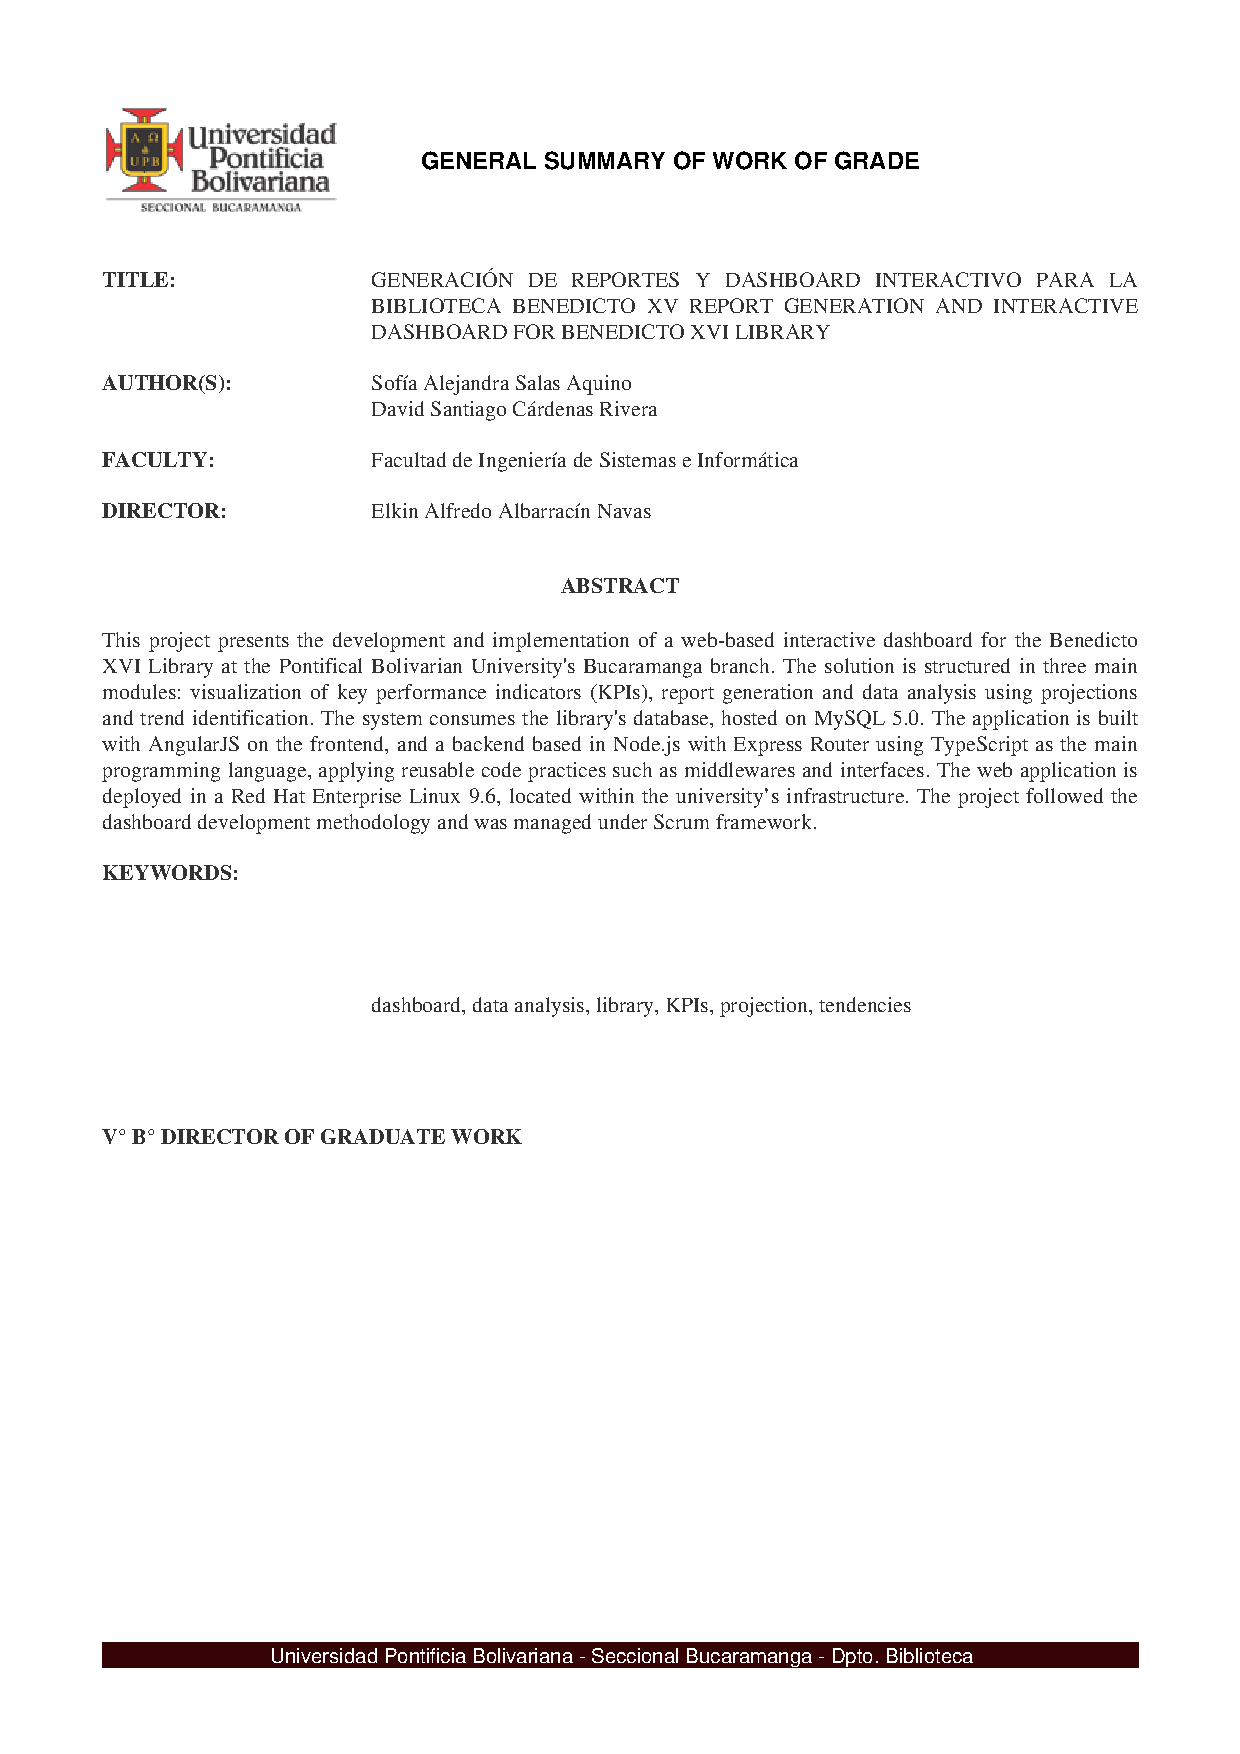
\includepdf[pages=-, pagecommand={\thispagestyle{fancy}}]{pdf_resumes/resumening.pdf}

\newpage
\section*{GLOSARIO}
\textbf{CTIC: } Centro de tecnologías de información y comunicaciones

\vspace{0.1cm}
\textbf{DBSM: } Database Management System (Sistema de Gestión de Base de Datos).

\vspace{0.1cm}
\textbf{DDC: } Clasificación Decimal Dewey

\vspace{0.1cm}
\textbf{IEEE: } Institute of Electrical and Electronics Engineers. 

\vspace{0.1cm}
\textbf{ISO: } International Organization for Standardization.

\vspace{0.1cm}
\textbf{KPI: } Key Performance Indicator (Indicador Clave de Desempeño). 

\vspace{0.1cm}
\textbf{SNIES: } Sistema Nacional de Información de la Educación Superior (Colombia). 

\vspace{0.1cm}
\textbf{SQL: } Structured Query Language. 

\vspace{0.1cm}
\textbf{TIC: } Tecnologías de la Información y la Comunicación.

\vspace{0.1cm}
\textbf{UMUX: } Usability Metric for User Experience.

\vspace{0.1cm}
\textbf{UPB: } Universidad Pontificia Bolivariana.

\vspace{0.1cm}
\textbf{UX: } User Experience (Experiencia de usuario). 
% Upload resumes in pdf_resumes folder
% THIS MUST BE SIGNED BY DIRECTOR
% visit: https://herramientasbib.bucaramanga.upb.edu.co/resumenesp
% visit: https://herramientasbib.bucaramanga.upb.edu.co/resumening

%%%%INYECTAR PDF

%
\includepdf[pages=-, pagecommand={\thispagestyle{fancy}}]{pdf_resumes/resumenesp.pdf}
%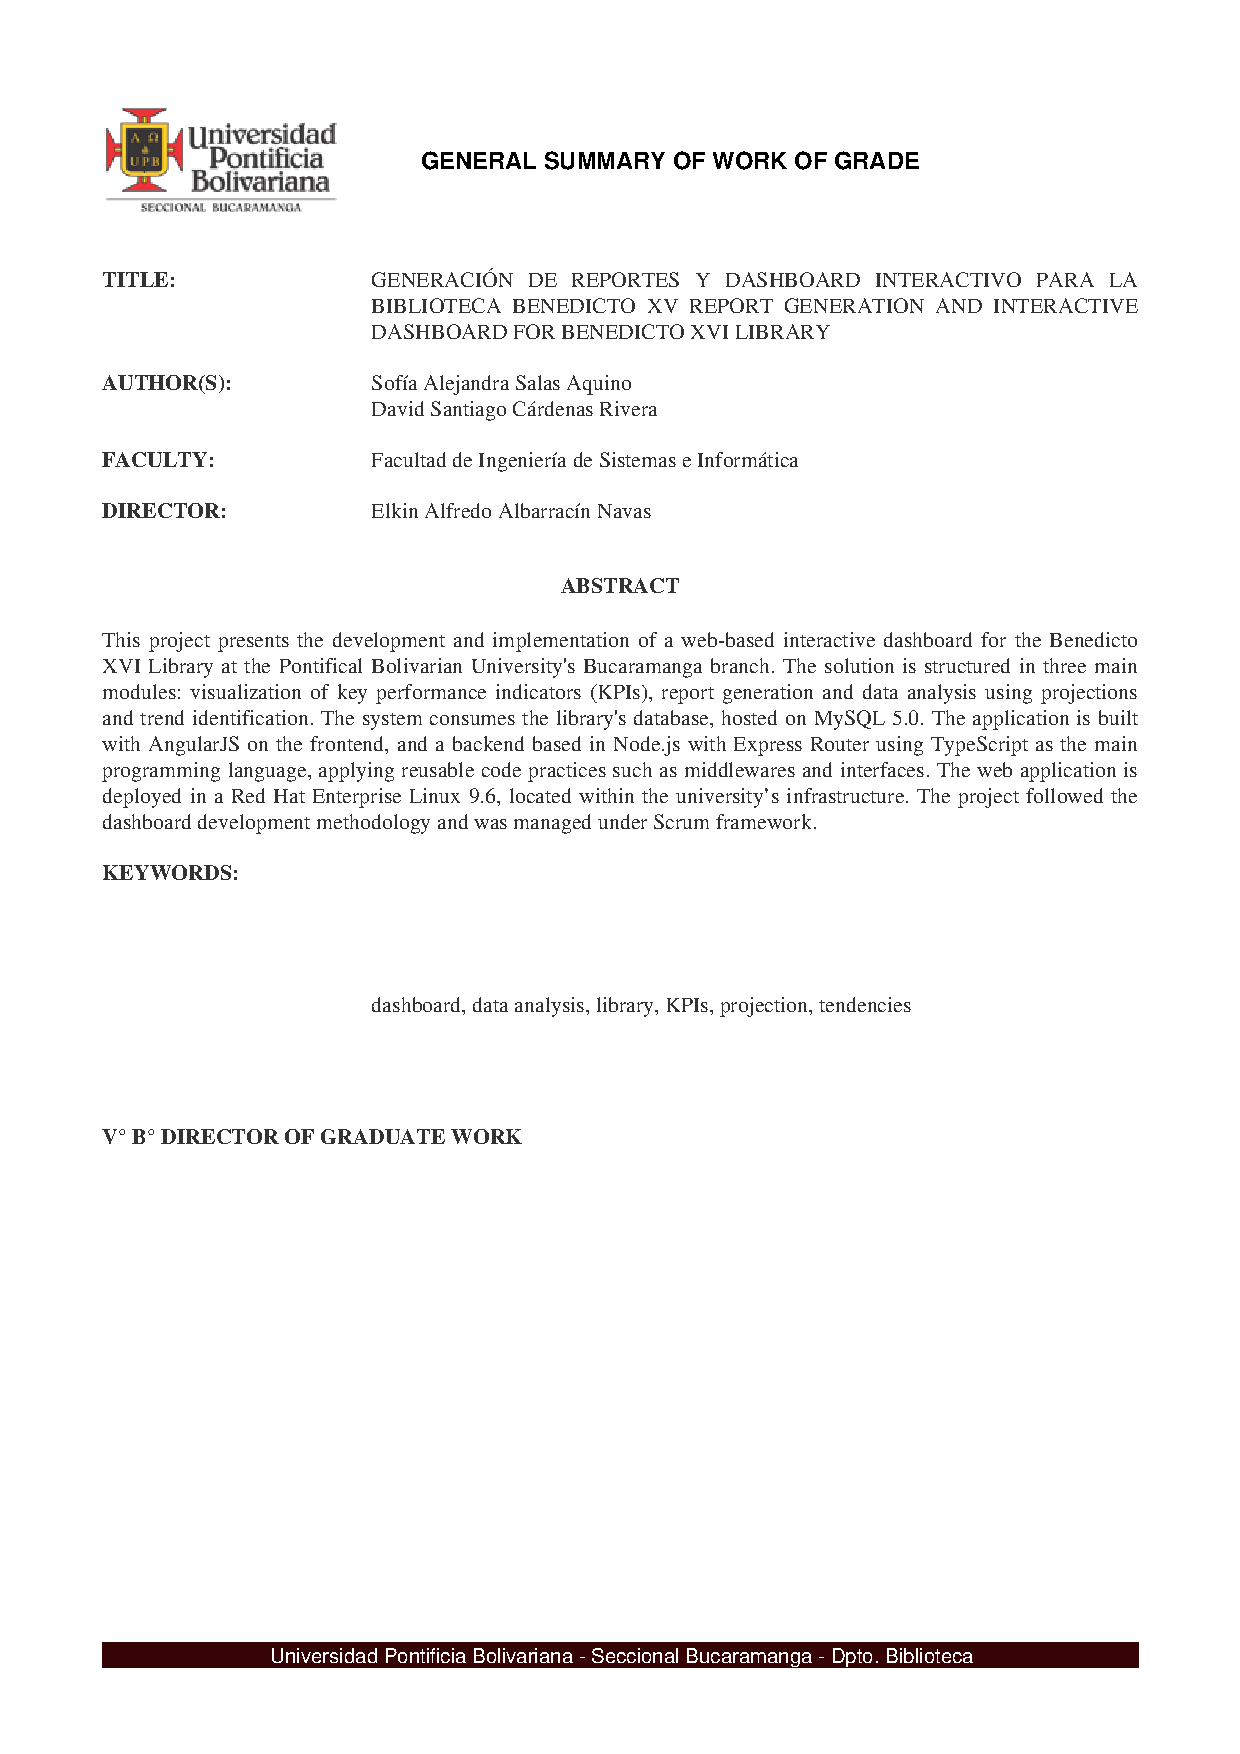
\includepdf[pages=-, pagecommand={\thispagestyle{fancy}}]{pdf_resumes/resumening.pdf}

% Introducción
\newpage
\section{INTRODUCCIÓN}

La biblioteca Benedicto XVI de la Universidad Pontificia Bolivariana cuenta con una base de datos relacional donde se registra y almacena datos como el uso de material bibliográfico diariamente, inventario físico actualizado, préstamos de usuarios y consultas. Sin embargo, la biblioteca no cuenta con un sistema para el análisis y revisión de estos datos, llevando al personal a realizar consultas en el departamento de CTIC de la universidad para la disposición de los datos; esto lleva tiempo y es un proceso manual, dificultando la toma de decisiones estratégicas basada en datos reales. 

\vspace{0.3cm}
Con el fin de superar estas limitaciones, el presente proyecto propone el diseño, desarrollo y despliegue de un dashboard interactivo para la visualización y análisis de datos extraídos y procesados de la base de datos de la biblioteca.

\vspace{0.3cm}
Se adoptó el marco de trabajo \textit{Scrum} para el desarrollo del sistema, presentando ciclos iterativos de entrega y retroalimentación continua por parte de la Jefatura de Biblioteca. Aparte, se adaptó la metodología de desarrollo de dashboards estratégicos Hariyanti, dividiendo el proyecto en cinco fases: Identificación de necesidades, planeación, diseño del prototipo, desarrollo e implementación. 

\vspace{0.3cm}
La implementación del dashboard interactivo permite a la biblioteca Benedicto XVI la visualización de su estado actual  por medio de la visualización, análisis, proyección y comparación de datos estadísticos relacionados con la información recolectada diariamente en la base de datos, soportando la toma de decisiones estratégicas por parte de los administrativos con datos confiables y la exploración de las tendencias que existen entre los usuarios. 


% Planteamiento del problema
\newpage
\section{PLANTEAMIENTO DEL PROBLEMA}

En la actualidad, el creciente uso de herramientas tecnológicas han generado que en cualquier ámbito, y sobretodo el bibliotecario, exista la necesidad de optimizar el procesamiento, análisis y reporte, de información estadística. En este sentido, algunas instituciones han implementado sistemas automatizados que faciliten la toma de decisiones basadas en datos. 

\vspace{0.3cm}
En el contexto de la Universidad Pontificia Bolivariana, campus Bucaramanga, se ha identificado que el módulo actual de estadísticas de la Biblioteca Benedicto XVI presenta limitaciones notables, entre las que se destacan: la generación manual de reportes, donde el proceso de elaboración de reportes se realiza en formatos de \textit{queries} directos a la base de datos para poder suplir con los objetivos del negocio o algunos otros casos de uso; la falta de visualización interactiva con ausencia de \textit{dashboards}, en el sistema web ya existente, impidiendo una interpretación dinámica y en tiempo real de los datos para distintos factores, limitando la capacidad de respuesta de los usuarios administrativos a cargo de esto; así como también la falta de estadísticas, como gráficos y KPIs, que se alineen con los objetivos de la biblioteca.

\vspace{0.3cm}
Algunos estudios incluso evidencian la importancia de contar con sistemas automatizados para estadísticas y reportes. Por ejemplo, para la situación bibliotecaria en Colombia, el Censo de Bibliotecas Públicas realizado por el Cerlalc en 2011 reportó que, en instituciones de gran tamaño, se registraban promedios mensuales superiores a 150.000 visitas, lo que denota la necesidad de manejar de datos exactos que permitan gestionar eficientemente recursos bibliotecarios, encuadrados en posibles géneros, libros, etc \cite{CERLALC2011}. Además, en ciudades como Bogotá se han registrado aumentos significativos en la actividad de estos espacios; según datos de BibloRed \cite{BIBLORED2022}, en 2022 se alcanzaron 2.197.673 visitas, lo que representa un incremento del 24\% en comparación con 2021, demostrando que la demanda por estos servicios continúa en aumento y, por lo tanto, requiere de un sistema que aparte la operación manual repetitiva.

\vspace{0.3cm}
Otros estudios, contextualizados en el exterior, también evidencian esta misma tendencia. Tal es el caso de la Biblioteca Pública Provincial de Málaga, la cual registró 99.276 visitas en el periodo de enero a septiembre de 2024 \cite{SER_malaga2024}; o también en La Rioja, donde se reportaron aproximadamente 340.000 préstamos en 2023 entre 24 bibliotecas públicas \cite{SER_rioja2024}; así como el crecimiento del 14\% en el número de usuarios en la biblioteca de Ponferrada que ilustra su aumento en la demanda \cite{SER_ponferrada2025}.

\vspace{0.3cm}
Aunque estos datos provienen de bibliotecas públicas, son reflejo de tendencias generales que aportan elementos cuantitativos comparables con las necesidades que puede presentar una biblioteca universitaria. Para la automatización en bibliotecas universitarias, Arriola Navarrete y Tecuatl Quechol \cite{Arriola2011}, evidencian que la adopción de sistemas integrados de automatización tipo SIAB (Sistemas Integrales de Automatización de Bibliotecas) permite optimizar procesos, mejorar la calidad del servicio y mejorar la toma de decisiones para las distintas áreas con las que cuenta.

\vspace{0.3cm}
Gracias a esto, se puede determinar que, basado en las necesidades de la Universidad Pontificia Bolivariana: Seccional Bucaramanga, nace la pregunta problema de: ¿Cómo se puede implementar un sistema que permita la generación automatizada de reportes y que a su vez cuente con herramientas interactivas para visualizar estadísticas sobre el préstamo y uso de libros en sala, integrando estos servicios al módulo existente de la Biblioteca Benedicto XVI en la Universidad Pontificia Bolivariana: Seccional Bucaramanga?

% Justificación
\newpage
\section{JUSTIFICACIÓN}
Actualmente, la generación de reportes en la biblioteca se realiza mediante la herramienta Microsoft Excel, específicamente a través del apartado de obtención de datos desde otras fuentes, lo que establece una conexión directa con la base de datos de la biblioteca. Estas consultas se manejan utilizando el lenguaje \textit{SQL}; sin embargo, no hay personal capacitado en la biblioteca para realizar esta tarea, lo que convierte la generación de reportes mensuales en un proceso tedioso y obliga al personal a solicitar constantemente la ayuda de externos y del departamento TIC (conocido como CTIC) de la institución. Por esta razón, la implementación de un servicio para la generación automatizada de reportes es una necesidad que el personal de la biblioteca ha manifestado al equipo de trabajo.

Por otro lado, la biblioteca no cuenta con herramientas para conocer indicadores estadísticos, tales como cuáles son los libros más usados en un determinado período, cuáles son los estudiantes que más utilizan el servicio de biblioteca, cuáles son los géneros y subgéneros de libros más consultados, y qué roles hacen mayor uso de los libros. Por este motivo, se ha planteado la implementación de un \textit{dashboard} interactivo, que permita, mediante la visualización de indicadores estadísticos, que la biblioteca tome decisiones institucionales basadas en datos reales.

Además, la biblioteca cuenta con un servicio web llamado ''estadística de libros'', en el que se registran los libros utilizados día a día por los estudiantes. El personal de la biblioteca manifestó estar familiarizado con el uso de este servicio y solicitó la implementación de las funcionalidades descritas en este apartado.

% Objetivos
\newpage
\section{OBJETIVOS}

\subsection{Objetivo general}

Desarrollar un sistema web que permita la generación automatizada de KPIs apoyado en un \textit{dashboard} interactivo para visualizar estadísticas sobre el préstamo y uso de libros en sala, e integrar estos servicios al módulo existente de estadística de libros de la biblioteca Benedicto XVI en Universidad Pontificia Bolivariana, campus Bucaramanga.

\subsection{Objetivos específicos}

\begin{itemize}
\item Definir  las historias de usuario para la especificación de requisitos funcionales y no funcionales, basándose en los módulos de generación de reportes y \textit{dashboard.}
\item Diseñar las funcionalidades para el módulo de generación de reportes y \textit{dashboard.}
\item Desarrollar las funcionalidades teniendo como base los diseños realizados.
\item Integrar las funcionalidades en la infraestructura tecnológica de la Universidad Pontificia Bolivariana seccional Bucaramanga.
\end{itemize}


% Marco referencial
\newpage
\section{MARCO REFERENCIAL}

\subsection{Antecedentes}

\stepcounter{mytablecounter} % Incrementa el contador personalizado

%%%%%%%%%%%%%%%%%%%%%%%%%%%%%%%%

En el artículo \textit{Designing Dashboard Visualization for
Heterogeneous Stakeholders} \cite{DashboardHeterogeneous}, se trata el caso en donde la biblioteca central ITB, ubicada en la universidad ITB en Indonesia plantea la necesidad de la implementación de un \textit{dashboard} para la toma de decisiones administrativas, y análisis estadísticos realizados por \textit{Stakeholders} con diferentes intereses y finalidades\cite{MeaningHeterogeneousStakeholders}. Se planteó una metodología para el desarrollo de tableros ejecutivos, la cual consiste en identificar las necesidades de la organización (esta fase involucra la identificación de los \textit{stakeholders}, posibles KPIs en los que estos estarían interesados, e identificar las necesidades de cada uno). Posteriormente, se diseña el prototipo según los intereses de la biblioteca. En el diseño realizado, se utiliza la información de tres bases de datos existentes de la biblioteca, en donde se almacena respectivamente: la información del inventario de libros, los préstamos y las visitas. Luego, se realiza la implementación del diseño. El producto final fue una página en donde se incluía la cantidad de títulos por cada género literario, el costo promedio por asignatura, y la temática de libros más prestados según cada facultad.
Esto permitió ayudar a los \textit{stakeholders} a entender los intereses de cada facultad, y así prestar un servicio más acertado\cite{DashboardHeterogeneous}.
Para medir la satisfacción de los \textit{stakeholders} con el producto final, se usó la medida UMUX, la cual mide la efectividad del producto, eficiencia, satisfacción y facilidad de uso. La evaluación obtuvo como resultado 89.3, de un resultado máximo de 100. Se concluyó que el resultado de eficiencia en la prueba UMUX fue más bajo que los otros debido a que la biblioteca nunca ha tenido un \textit{dashboard}, y la aglomeración de componentes en una página puede producir resultados bajos. Sin embargo, según el puntaje de la prueba, se constató que el  \textit{dashboard} cumplió con los objetivos planteados.\cite{DashboardHeterogeneous}

El software de código abierto para el manejo de bibliotecas Koha\cite{KOHA}, presta una solución para la generación de reportes basándose en la información registrada en la base de datos relacional que el software usa para el almacenamiento de los datos\cite{koha_manual_custom_reports}. Sin embargo, estos reportes quedan guardados bajo el aplicativo, y no se pueden exportar a otro formato. Según la documentación sobre reportes de Koha\cite{koha_manual_custom_reports}, existen dos opciones para la generación de reportes: \textit{guided reports wizard} y por medio de comandos \textit{SQL}. El \textit{guided reports wizard} presenta una interfaz gráfica en donde el usuario puede seleccionar las columnas y atributos que debe tener el reporte.

Por medio del \textit{guided reports wizard}, los reportes se pueden generar en un formato mensual, anual y un periodo de tiempo especificado por el usuario. Se debe seleccionar el año inicial en cualquiera de los casos. En este momento, solo existe el tipo de reporte tabular, el cual genera una tabla. Posteriormente, el usuario debe seleccionar las columnas que quiere en el reporte según la información presente en la base de datos. Las opciones se muestran en un menú plegable. Luego de esto, se guarda el reporte. Koha es usado por más de 50 instituciones educativas en Colombia\cite{kohaDatosColombia}.

En el artículo \textit{Implementation of Automated Library Management System in the School
of Chemistry Bharathidasan University using Koha Open Source Software}\cite{colegioKoha} se expone la creciente necesidad para adoptar técnicas modernas para el manejo de biblioteca debido a que “Los métodos antiguos para mantener bibliotecas dejaron de ser dinámicos y eficientes'', fundamentado en el constante crecimiento del material bibliográfico y la lenta respuesta que los métodos antiguos proveían con respecto a sistemas automatizados de manejo.\cite{colegioKoha}. 

Por este motivo, se decidió realizar pruebas para la posible implementación del software libre \textit{Kohan}, resaltando el módulo de reportes para los detalles relacionados con los libros vencidos, el monto total pagado y el monto total cancelado, actividades de los usuarios relacionadas con libros vencidos, multas por atraso, multas pagadas y multas pendientes. Después de las pruebas, se concluyó que el software Koha es más adecuado para el manejo y gestión de la biblioteca, que la realización de las actividades manualmente.

\subsection{Marco teórico}
La toma de decisiones basada en datos se ha convertido en una necesidad para instituciones como las bibliotecas. La implementación de este tipo de sistemas de estadísticas y reportes, para usuarios administradores como los que se retratan en este proyecto, permite optimizar la gestión de recursos, tener transparencia en el manejo de datos y facilitar la evaluación del desempeño de distintos ámbitos de la biblioteca. 

\vspace{0.3cm}
Esta sección desarrolla los fundamentos teóricos en los que se basa el proyecto, abarcando la importancia de la estadística, el uso de \textit{dashboards}, la relevancia de los reportes, así como su generación sistematizada, y la elección del formato XLSX como herramienta para la entrega de los mencionados.

\vspace{0.3cm}
\subsubsection{\textit{Dashboards} para la toma de decisiones}
Según Zingde, S. y Shroff, N. \cite{zingde2020role}, para un usuario, la información poco visual y más textual, llega a dificultar la toma de decisiones, sobretodo en un mundo moderno que es cada vez más competitivo y en el que la demanda de los clientes crece a ritmos relativamente rápidos. Esta acción que, en pocas palabras, es una resolución de problemas que enfrenta la organización, requiere que tenga como prioridad aspectos que permitan la optimización de recursos y la entrega de servicios a tiempo.

\vspace{0.3cm}
Para que estos elementos esenciales se puedan cumplir, las organizaciones buscan la forma en la que la información sea relevante y confiable para poder cumplir con los objetivos del negocio. Es por ello por lo que las organizaciones se ven obligadas a implementar herramientas que permitan cumplir con lo requerido, siendo una de estas el \textit{dashboard}.

\vspace{0.3cm}
Los \textit{dashboards}, según como lo establece Zingde, S. y Shroff, N. \cite{zingde2020role}, cumplen con tener propósitos: tal como la medición de rendimiento, análisis del uso de los recursos, la planificación y la predicción; capacidades: donde se encuentra el análisis de escenario y los análisis predictivos; y expectativas: como la confianza y precisión de la información, así como el acceso a información en cualquier tiempo que se necesite. Se puede ver más detallado estos factores en la figura \ref{fig:dashboard_pce}.

\begin{figure}[htpb] 
	\centering
	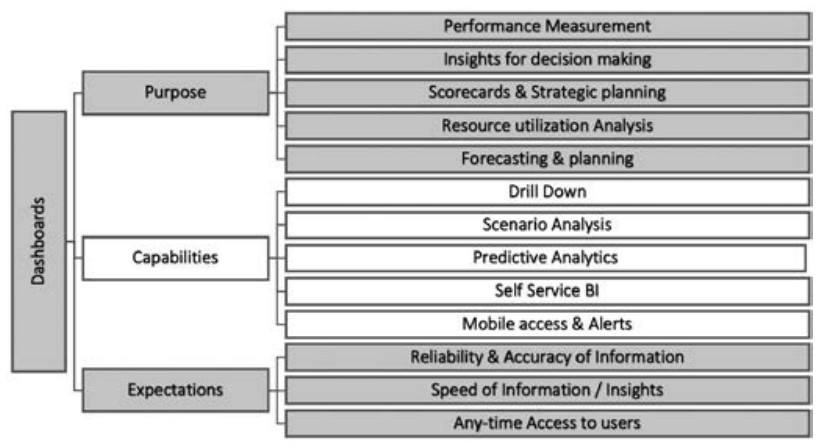
\includegraphics[width=0.8\linewidth]{img/dashboards_pce.jpg}
	\vspace{-1mm}
	\caption[Definición de Dashboard]{\textit{Dashboards - Propósito, Capacidades y Expectativas}. Imagen tomada de \cite{zingde2020role}.}
	\label{fig:dashboard_pce} 
\end{figure}

\vspace{0.3cm}
En un plano general, estos tienen como rol otorgar visualización de los datos, impactando en la velocidad y la calidad en la toma de decisiones, conteniendo aspectos como la capacidad de interacción con estos para la obtención de más detalles sobre la información de la que se intenta indagar. Asimismo, tiene otros propósitos como el de permitir un manejo óptimo en las mediciones de los KPIs y los rendimientos de distintos módulos relacionados con los objetivos del negocio.

\vspace{0.3cm}
Por el lado del diseño de estos \textit{dashboards}, para que puedan cumplir con este rol, deben de usar visuales adecuadas, así como tener ubicaciones pertinentes, ajustadas según las necesidades y prioridades de la organización. La información clave siempre debe estar arriba del todo, le debe seguir información relacionada a esta y los componentes que contengan mayor detalle y datos textuales, deben ubicarse en la parte inferior \cite{zingde2020role}.

\vspace{0.3cm}
\subsubsection{Generación de reportes}
Según \textit{Intuit Mailchimp} \cite{mailchimp_report} la generación de los reportes automáticos trata sobre la recolección y generación específicas de información en un cierto rango de tiempo establecido. Esta automatización de reportes permite crearlos para distintos propósitos, ya sea monitorear operaciones del negocio, acceder a datos actualizados, entre otros.

\vspace{0.3cm}
Este sistema tiene relevancia, debido a que permite que haya consistencia sobre los datos que se intentan reportar; asegura que los datos sean exactos y acertados, obteniendo estos de fuentes directas como una base de datos, permite tomar decisiones ''en tiempo real''. Además, lo convierte en un aspecto de suma importancia, debido a que hace eficiente el trabajo de generar informes que requieran personas/organizaciones que los requieran, tales como los \textit{stakeholders} de esa organización \cite{mailchimp_report}.

\vspace{0.3cm}
Asumiendo que se necesitase un reporte para un área específica, en un rango de tiempo determinado, sin un sistema de generación de reportes automatizado, este proceso podría tomar tiempos de medio día, hasta incluso una semana completa, dependiendo de la exigencia en las necesidades, según lo afirma FineReport \cite{finerep_automatedrep_2024}. A final de cuentas es un trabajo repetitivo que manualmente requiere de mucha labor y es un aspecto que es esencial cuando se manejan datos en los distintos casos de uso dentro de una organización como lo es una biblioteca. Con un sistema de reportes automatizado, es posible generarlos en el formato que se desee, así como las posibilidades de añadir otros módulos, que faciliten aún más el proceso, permitiendo realizar diferentes acciones con estos, como lo puede ser un sistema de automatización que le permita  enviar estos reportes a través de distintos medios cada cierta frecuencia de tiempo.

\vspace{0.3cm}
Usualmente, para la generación de reportes se deben contemplar los siguientes aspectos:

\begin{itemize}
    \item El o los formatos en los que se puede generar.
    \item Las plantillas ajustadas para los formatos que se establecieron.
    \item Las posible columnas de datos a incluir.
    \item Una interfaz que permita comunicar con algún sistema/componente que obtenga la información de la base de datos, realice el debido procesamiento y retorne la información tratada para la generación del reporte.
    \item Librería/algoritmo para la generación de reportes, que reciba cierto tipo de datos, usando lenguajes de programación y \textit{frameworks} que se ajusten a las necesidades del negocio.
\end{itemize}

\subsection{Marco conceptual}

%%%%%%%%%%%%%%%%%%%%%%%%%%%%%%%%%%%%%%%%%%%%%%%%%
    \subsubsection{Stakeholders:} Hace referencia a cualquier grupo de personas o individuo que puede afectar o ser afectado por el logro de los objetivos de la institución\cite{freeman1984strategic}. Dentro del proyecto, los \textit{Stakeholders} corresponderían al personal de la biblioteca Benedicto XVI, la facultad de ingeniería de sistemas e informática de la UPB, y los encargados del proyecto.  
    \subsubsection{Modulo de estadística: } corresponde al servicio web donde el personal de biblioteca Benedicto XVI registra los libros consultados en sala día a día. Estos se registran por medio de escaneo del código de barras del libro, el cual está asociado al número de inventario en la base de datos de la biblioteca.

    \subsubsection{Libros usados en sala: } Se definen como los libros que los usuarios de la biblioteca Benedicto XVI usan día a día dentro del establecimiento. En la biblioteca se tiene la indicación de dejar los libros usados sobre las mesas de trabajo, para que estos posteriormente sean registrados en el módulo de estadística.
    
    \subsubsection{Libros prestados: }Corresponde a los libros que los usuarios de la biblioteca Benedicto XVI solicitan por medio del servicio de préstamo. Para el préstamo de libros se dispone un periodo de un mes (plazo designado para el año 2025) en donde el estudiante está a cargo del material. Tres días antes de la fecha de vencimiento del plazo, se envía un correo al estudiante para que este realice la renovación del libro por el servicio web de \textbf{Alejandría}, o se acerque al establecimiento a renovarlo. 

    
    \subsubsection{Alejandría: }Portal web en donde los usuarios de la biblioteca pueden realizar consultas sobre el catálogo disponible. La búsqueda se puede realizar por Título del material, autor y palabras claves. Existe un apartado de búsqueda ''específica'', en donde el usuario puede escoger por cuál parámetro desea realizar la búsqueda, teniendo como opciones: Inventario (realiza una búsqueda en el inventario por el código del libro en la base de datos), ISBN, Signatura topográfica, Clave de autor, año de edición.
    
    \subsubsection{Ejemplares de libros: } Corresponde a la cantidad de ejemplares de un solo libro de libros que existe en el inventario de la biblioteca Benedicto XVI.

\subsubsection{Decimal Dewey Classification (DDC):} Sistema de clasificación bibliográfica que organiza recursos bibliográficos mediante números decimales, estos números corresponden a géneros literarios y subgéneros, facilitando su ubicación en bibliotecas. El DDC es el sistema de clasficación más usado en el mundo. Más de 135 países usan el DDC para organizar su material bibliográfico, y este ha sido traducido a más de 30 idiomas\cite{oclc_dewey}. Se compone de 10 clases principales. En la siguiente tabla, se indica el código numérico principal y su clasificación correspondiente:
%%%%


%%%%
\addcontentsline{lot}{table}{\protect\numberline{\themytablecounter}Diez clases principales de DDC }
\begin{table}[htpb]
    \centering
    \caption[Decimal Dewey Classification (DDC)]{\bfseries DIEZ CLASES PRINCIPALES DE DDC}
    \label{tab:clasificacion_decimal}
    \begin{tabular}{lll} \hline
     
        \textbf{Código} & \textbf{Clase} \\ \hline
        000 & Conocimiento general \\ 
        100 & Filosofía \& psicología\hspace{7.5cm} \\ 
        200 & Religión \\ 
        300 & Ciencias sociales \\ 
        400 & Lenguaje \\ 
        500 & Ciencias naturales \\
        600 & Tecnología \\ 
        700 & Artes \& recreación \\ 
        800 & Literatura \\ 
        900 & Historia \& geografía \\ \hline
    \end{tabular}
    \vspace{2mm}
    \newline
    \small{Estas son las diez primeras clasificaciones en el sistema Decimal Dewey.}
\end{table}


%%%%


Después de esta clasificación, se encuentra la clasificación llamada ''las 100 divisiones'', indicando el equivalente en subgéneros por cada decena. Posteriormente, se encuentra la clasificación ''las mil secciones'', el cual enseña la equivalencia de cada unidad. En la biblioteca Benedicto XVI, se usa el DDC para la clasificación de los libros. De esta forma, se puede conocer el género de un libro dentro de la biblioteca, y encontrar su ubicación en los pasillos. 


  \subsubsection{Dashboard: } Es una muestra visual de la información más importante para conseguir uno o más objetivos, diseñado y ajustado en una vista de una sola ventana de navegador para que la información pueda ser monitoreada a la vista. Esta información se muestra por medio de gráficos estadísticos\cite{few2006information}. Por medio de entrevistas con el personal encargado de la biblioteca Benedicto XVI, se determinó la necesidad de un \textit{Dashboard} para la visualización de información relacionada con los libros más usados, estudiantes que realizan más préstamos de libros, géneros u subgéneros de libros más consultados.  

  \subsubsection{Reportes: }Documentos que resumen y comunican datos y métricas de procesos o actividades realizadas en una institución\cite{ibm_reports_2018}. En la biblioteca Benedicto XVI, los reportes se realizan en función de cuáles fueron los libros usados en sala en cierto periodo de tiempo, libros perdidos y descartados del inventario, cuál material bibliográfico no ha sido prestado en cierto periodo de tiempo.

    \subsubsection{KPI (Key Performance Indicators)} es un indicador medible que indica el desempeño de una institución relación con los objetivos establecidos o empresariales\cite{marr2012key}. Para la identificación de KPIs claves para la biblioteca Benedicto XVI, se deben determinar sus objetivos finales. 
    
  \subsubsection{UMUX} Es una escala para medir la usabilidad percibida por el usuario final de un aplicativo. Se rige bajo la definición de usabilidad de la ISO 9241-11\cite{finstad2010usabilityUMUX}. Cuenta con cuatro escalas, especificadas en la siguiente tabla: 
% Entrada manual en la Lista de Tablas
\addcontentsline{lot}{table}{\protect\numberline{\themytablecounter}Indicadores de UMUX}

\begin{table}[htpb]
    \centering
    \caption[Indicadores de UMUX]{\bfseries INDICADORES DE UMUX}
    \label{tab:evaluacion_sistema}
    \begin{tabular}{lll} \hline
        \textbf{Indicador} & \textbf{Descripción} \\ \hline
        Efectividad  & Este sistema cumple con mis requerimientos. \\
        Satisfacción & Este sistema es una experiencia frustrante. \\ 
        Facilidad    & Este sistema es sencillo de usar. \\ 
        Eficiencia   & He pasado mucho tiempo corrigiendo cosas con este sistema. \\ \hline
    \end{tabular}
    \vspace{2mm}
    \newline
    \small{Indicadores empleados en la escala UMUX \cite{finstad2010usabilityUMUX}.}
\end{table}



Cada una de estas categorías es medida en una escala del 1 al 7, siendo uno ''Extremadamente en desacuerdo'', y siete ''Extremadamente de acuerdo''. Posteriormente, el resultado de la prueba UMUX es la suma de los 4 ítems dividivo en 24 y posteriormente, multiplicado por 100\cite{finstad2010usabilityUMUX}. Por medio del UMUX, se puede realizar la prueba de usabilidad con el usuario final de la biblioteca y obtener un resultado medible.

  \subsubsection{Gráfico de barras: } Representación visual que utiliza barras rectangulares para comparar valores entre diferentes categorías.\cite{healy2018data}. En un estudio realizado por Heer y Bostock\cite{heer2010crowdsourcingESTUDIOGRAFICAS}, se determinó que el desempeño del entendimiento de la información representada en un gráfic era mejor en la gráfica de barras que en ocho tipos de gráfica distinta, en donde se encontraba el gráfico de torta, y el gráfico de áreas apiladas. Para el \textit{dashboard} de la biblioteca Benedicto XVI, se procura utilizar este tipo de gráfica para la representación de los datos.


   \subsubsection{Extensión XLSX: } Formato de archivo de Microsoft Excel basado en XML para almacenar hojas de cálculo y datos.\cite{microsoft_xlsx_2019}. Este será el formato de archivo que será usado para la generación de reportes para la biblioteca Benedicto XVI.

  \subsubsection{Bases de datos relacional: } Sistemas de gestión de bases de datos que organiza la información en tablas compuestas por filas y columnas, estableciendo relaciones entre ellas mediante claves primarias y claves foráneas\cite{ibm_relational_databases}.Esta estructura permite un acceso eficiente a los datos y facilita operaciones como la consulta, inserción, actualización y eliminación de información\cite{ionos_relational_databases}.   La base de datos actual de la biblioteca Benedicto XVI es una base de datos relacional, lo que indica que sus tablas están relacionadas entre sí.

  \subsubsection{Backend} Parte del desarrollo de software que se encarga del procesamiento de datos, la lógica de negocio y la comunicación con bases de datos, operando en el servidor \cite{ibm_backend_2020}. Para el desarrollo de las funcionalidades referentes a la generación de reportes y el \textit{dashboard}, se debe desarrollar un \textit{backend} para establecer la lógica de negocio.

  \subsubsection{ISO: } corresponde a la  organización Internacional de Normalización, responsable de establecer estándares internacionales en diversos campos\cite{iso_standards_2019}. Específicamente, se plantea la ISO 11620:2023 para los indicadores de desempeño de una librería\cite{iso11620_2023Library}.  

  \subsubsection{Filtro en generación de reportes} Funcionalidad que permite seleccionar y refinar la información que se incluirá en un reporte, basándose en criterios específicos \cite{ibm_report_filter_2021}.
%%%%%%%%%%%%%%%%%%%%%%%%%%%%%%%%%%%%%%%%%%%%%%%
\subsection{Marco tecnológico}

    \subsubsection{TypeScript:} Lenguaje de programación desarrollado por Microsoft que extiende JavaScript mediante la adición de tipado estático y características orientadas a objetos. TypeScript permite detectar errores durante la fase de compilación y mejora la legibilidad y mantenibilidad del código\cite{typescript_2020}.
  
  \subsubsection{Node.js:} Entorno de ejecución basado en el motor V8 de Google que permite ejecutar código JavaScript del lado del servidor. Node.js cuenta con un modelo de entrada/salida no bloqueante y orientado a eventos\cite{nodejs_2020}.
  
  \subsubsection{Express:} Framework para Node.js que simplifica el desarrollo de aplicaciones web y la creación de APIs RESTful. Express proporciona una estructura para la definición de  rutas, gestión solicitudes y respuestas HTTP \cite{express_framework_2020}.

    \subsubsection{Patrón Singleton:} El patrón Singleton garantiza que una clase tenga una única instancia y proporciona un punto de acceso global a dicha instancia. Este patrón asegura que la instancia se reutilice en toda la aplicación \cite{gamma1994design}.
  
  \subsubsection{Patrón Abstract Factory:} El patrón Abstract Factory permite la creación de familias de objetos relacionados sin especificar sus clases concretas, promoviendo el desacoplamiento entre la creación de objetos y su uso \cite{gamma1994design}.



\subsection{Marco institucional}


El desarrollo del proyecto de generación de reportes de biblioteca y el \textit{dashboard} intereactivo se realiza como un servicio para la biblioteca Benedicto XVI de la Universidad Pontificia Bolivariana, Seccional Bucaramanga.

Esta biblioteca tiene como misión:
\textit{''Facilitar la formación integral de los docentes, investigadores, estudiantes y personal administrativo de la Universidad Pontificia Bolivariana Seccional Bucaramanga, apoyando las actividades fundamentales de la UPB en docencia, investigación y promoción social, mediante la prestación de servicios bibliográficos pertinentes y de alta calidad.''}\cite{UPB_Biblioteca}

Su visión es:
\textit{''Ser el eje de toda la actividad académica, facilitando la adquisición del conocimiento mediante el uso adecuado de tecnologías avanzadas de información y comunicación para la difusión de información bibliográfica especializada a docentes, investigadores, estudiantes, personal administrativo de la UPB y entidades asociadas. La biblioteca espera contar con personal altamente capacitado en los servicios que ofrece y disponer de una infraestructura confortable que proporcione un ambiente adecuado para la consulta, lectura e investigación.''} \cite{UPB_Biblioteca}






%%%%%%%%%%%%%%%%%%%%%%%%%%%%%%%%%%


% Metodología
\newpage
\section{METODOLOGÍA}
\vspace{0.3cm}
El desarrollo del proyecto se basa en metodologías ágiles para el desarrollo de software, aplicando el marco de trabajo \textit{Scrum}. De estas metodologías se extraen elementos fundamentales como la planificación de sprints, la gestión del \textit{Product Backlog}, la revisión periódica del prototipo por parte del cliente y la adaptación continua a lo largo del proceso.
La metodología se divide en las siguientes cinco fases, en las que se detallan las actividades concretas que garantizan el cumplimiento de los objetivos del proyecto:

\subsection{Fase 1: Planificación}
\vspace{0.3cm}
En esta fase se definen los elementos iniciales y se establece la planificación general del proyecto. Se aborda la situación-problema identificando las necesidades del cliente mediante reuniones y entrevistas, se revisa la literatura relevante y se definen los objetivos del proyecto. Además, se establece la metodología de desarrollo basada en \textit{Scrum}, se crea el backlog priorizado, se elabora un cronograma para 4 semanas, se estima el presupuesto y se desarrolla el anteproyecto.

\subsection{Fase 2: Diseño}
En esta fase se diseña la solución, especificando las funcionalidades asignadas. Se identifican los casos de uso y se analizan los posibles flujos de interacción para que sean incorporados en el diseño del sistema.Esto corresponde a diseñar la interfaz de usuario y definir las funcionalidades relacionadas con la generación de reportes y la creación de un \textit{dashboard} interactivo.


\subsection{Fase 3: Desarrollo}

Se implementan las funcionalidades definidas en la fase de diseño utilizando tecnologías orientadas al desarrollo web, por medio de patrones de diseño.Aparte, se contempla el desarrollo de interfaces y componentes interactivos con frameworks oriendatos a diseño web. También se plantea la documentación y revisión de código para la mantenibilidad y escalabilidad del sistema. 

\subsection{Fase 4: Pruebas del Software}

En esta fase se valida, mediante pruebas, que el software cumpla con el flujo esperado. Se lleva a cabo una revisión por parte del cliente y, en función de su retroalimentación y de la evaluación de los requerimientos acordados, se retorna a la fase de diseño para realizar nuevas iteraciones del prototipo. Asimismo, se realizan reuniones de revisión y retrospectivas al final de cada sprint para identificar oportunidades de mejora continua.


\subsection{Fase 5: Integración y Despliegue en Producción}

Una vez que el software desarrollado cumpla con los requerimientos acordados con el cliente, se procederá a integrarlo en el entorno de producción de la Biblioteca Benedicto XVI.


\subsection{Integración del Marco de Trabajo \textit{Scrum}}

El marco de trabajo \textit{Scrum} se implementa a lo largo del proyecto, estructurándose en ciclos iterativos (sprints) de dos semanas aproximadamente. La integración se define de la siguiente manera:

\begin{itemize}
 \item \textbf{Planificación y Estimación:} En la reunión de planificación de cada sprint se organizan las actividades, se definen los objetivos del sprint y se seleccionan las tareas del \textit{Product Backlog} a abordar. Se estiman los tiempos y recursos necesarios para cada tarea, facilitando una planificación detallada. \cite{Schwaber2004,Cohn2005}.
 \item \textbf{Implementación:} Durante el sprint se desarrolla el proyecto, se establece la infraestructura tecnológica y se transforman los diseños en código funcional. Esta fase iterativa permite la entrega continua de incrementos de software operativos \cite{Sutherland2014}.
 \item \textbf{Revisión y Retrospectiva:} Al final de cada sprint se realiza una reunión de revisión en la que se evalúan los avances y se obtiene la retroalimentación del cliente. Posteriormente, en la retrospectiva, el equipo analiza el proceso de trabajo para identificar y aplicar mejoras en los siguientes sprints.
 \item \textbf{Lanzamiento:} Una vez culminados los sprints y validado el software, se procede al lanzamiento del producto. Este proceso incluye la integración final en producción, la comunicación de los resultados obtenidos y la documentación de los aprendizajes y éxitos alcanzados durante el proyecto.
\end{itemize}


\subsection{Adaptación de la metodología Hariyanti para el desarrollo de dashboards}

Se realizó una adaptación de una metodología preestablecida como la Hariyanti\cite{hariyanti-dashboard} para el desarrollo de \textit{dashboards} estratégicos. En esta se plantean aspectos claves que debe tener un \textit{dashboard estratégico} y cómo conseguirlos.

\vspace{0.3cm}
Se plantea como \textit{dashboard estratégico} un sistema que cumpla el propósito de brindar soporte a usuarios administrativos para la toma de decisiones empresariales basadas en la información presentada. Aparte, se alinea con los objetivos de la organización.\cite{hariyanti-dashboard}

\vspace{0.3cm}
\begin{figure}[htpb] 
	\centering
	\includegraphics[width=0.65\linewidth]{img/Metodología-hariyaki.png}
	\vspace{-1mm}
	\caption[adaptación de metodología propuesta por Hariyanti]{\textit{Metodología para el desarrollo de un dashboard adaptado de la metodología propuesta por Hariyanti\cite{hariyanti-dashboard}. Imagen propia.}}
	\label{fig:hariyanti} 
\end{figure}

En la metodología Hariyanti, se plantean las fases claves para el desarrollo de un dashboard:

\begin{itemize}
    \item \textbf{Identificación de necesidades: }Se identifican los objetivos de la organización, el tipo de dashboard, los usuarios objetivos y sus necesidades, y los posibles KPIs que brinden valor a la organización.
    \item \textbf{Planeación: }Se plantea las funcionalidades del dashboard, el contenido que este tendrá, y análisis de la información de los KPIs identificados.
    \item \textbf{Diseño del prototipo: }Diseño UX del dashborad y controles que este tendrá.
    \item \textbf{Revisión del prototipo: }Revisión y refinamiento del prototipo.
    \item \textbf{Implementación: }Consiste en la implementación del prototipo, selección de la tecnología a usar, integración con la fuente de información.
    
\end{itemize}

\vspace{0.3cm}
A partir de esto, se adaptaron las fases propuestas por Hariyanti, dando como fruto el esquema de trabajo propuesto en la figura \ref{fig:hariyanti}.
%%%%%%%%



\newpage
\section{\label{sec:cronograma}CRONOGRAMA DE ACTIVIDADES}
En la figura \ref{fig:cronograma} se puede observar el cronograma de actividades, dividido en 5 meses, donde se contemplan apartados como el diseño, desarrollo, implementación, pruebas del sistema, así como actividades para la gestión de la documentación. 

\vspace{0.3cm}
\begin{figure}[htpb] 
	\centering
	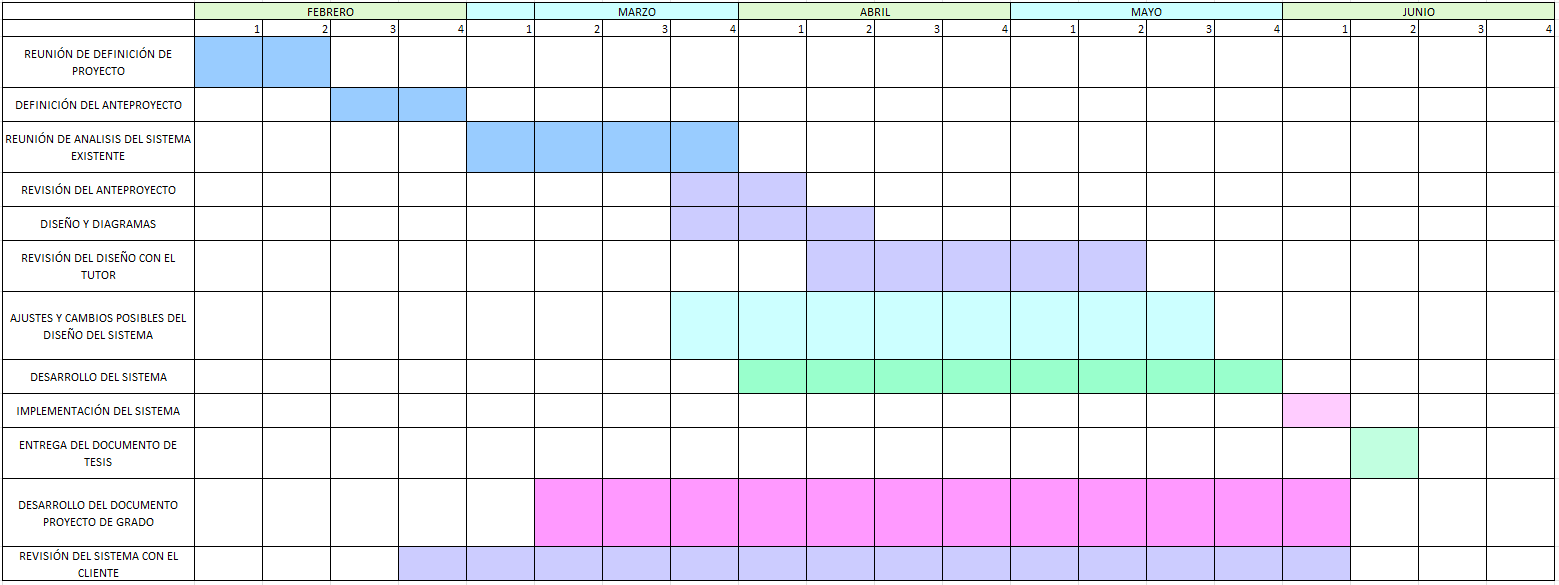
\includegraphics[width=0.8\linewidth]{img/Cronograma-ajustado-2.png}
	\vspace{-1mm}
	\caption[Cronograma de actividades]{\textit{Cronograma de actividades. Imagen propia}}
	\label{fig:cronograma} 
\end{figure}

\vspace{0.3cm}
Durante el desarrollo del proyecto, se mantuvieron reuniones semanales con el cliente para la verificación del avance de este, y realizar posibles correciones en el prototipo del producto y documentación. Aparte, en estas reuniones, se presentaban las dudas que iban surgiendo a medida del desarrollo del proyecto. Estas reuniones se realizaban los jueves a las 4 pm en la oficina de Jefatura de biblioteca, con la Jefa de biblioteca Yerika Alexandra Russi Porras. 


\newpage
\section{\label{sec:propiedadintelectual}PRESUPUESTO}
En la figura \ref{fig:presupuesto} se puede observar el presupuesto para el proyecto contemplando los apartados financieros para el recurso humano y los servicios.

\vspace{1cm}
\begin{figure}[htpb] 
	\centering
	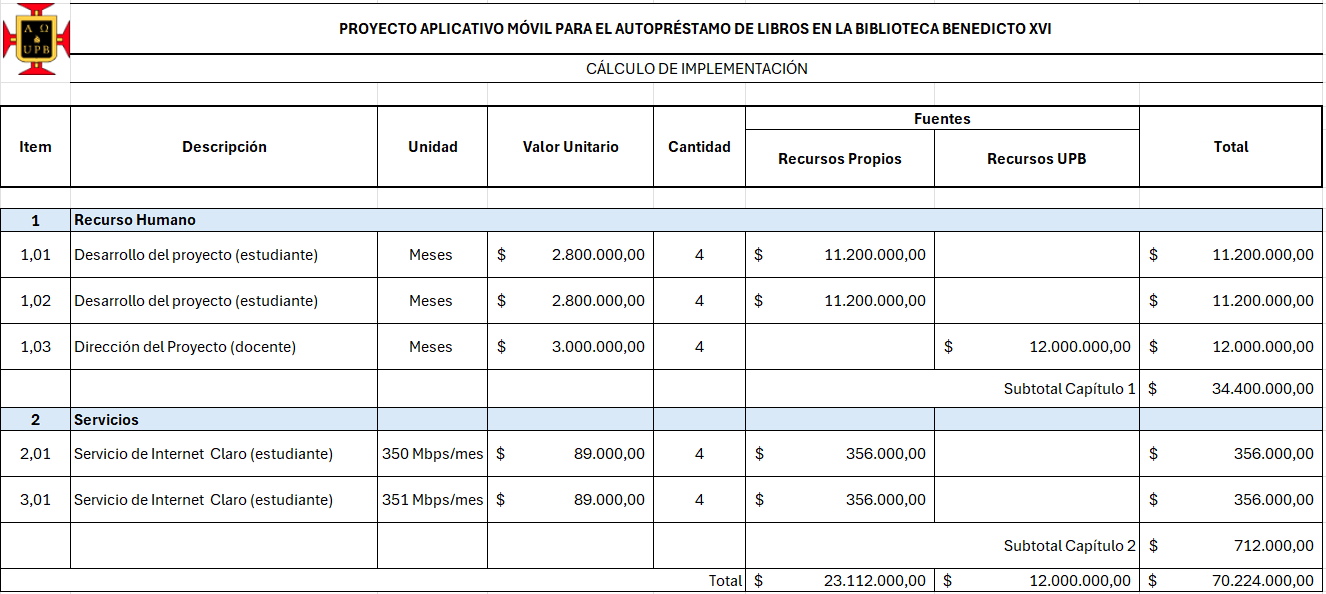
\includegraphics[width=0.9\linewidth]{img/presupuesto-inicial.png}
	\vspace{-1mm}
	\caption[Presupuesto para el proyecto.]{\textit{Presupuesto para el proyecto. Imagen propia}}
	\label{fig:presupuesto} 
\end{figure}



%%%%%%%%%%%%%%%%%%%%%%%%%%%%%%% Resultados

\newpage
\section{RESULTADOS}


\subsection{Primera fase: Identificación de necesidades}

\subsubsection{Identificar el objetivo de la biblioteca y la condición actual:}
Al momento de hacer un análisis del estado actual de la organización para el desarrollo de un dashboard, se concluye que la Biblioteca Benedicto XVI no ha presentado la implementación de un dashboard previamente, por lo tanto, los parámetros y especificaciones necesarios no están definidos. Por esta razón, se organizaron reuniones periódicas con el cliente, donde se abordaron discusiones sobre la identificación de necesidades para encontrar cuál sería la información clave para enseñar en el dashboard.

\vspace{0.3cm}
Se identifica que la biblioteca presenta una base de datos de más de cien millones de registros, sin embargo, un porcentaje grande de estos registros no poseían información fiable, es decir, hay campos vacíos, inconsistencias en la base de datos y poca o nula validación de entradas. Esto lleva a concluir que hay poca calidad en los datos. Aparte, la base de datos está poco normalizada, lo que dificulta el análisis. De un total de 132 tablas, el 31\% son consideradas inútiles, ya que son tablas de prueba, tablas sin registros, registros de prueba, o ya pasó su época de uso, como es el caso de las tablas relacionadas a la antigua hemeroteca, una sección de biblioteca que dejó de ser funcional alrededor del año 2021. 

\vspace{0.3cm}
En la página de Alejandría de la biblioteca Benedicto XVI, para usuarios administrativos, hay una sección que corresponde a generación de reportes a partir de la base de datos, sin embargo, al consultar con jefatura de biblioteca, se identificó que dentro de los reportes existentes, hacían falta algunos con referencia al estado del inventario. 

\vspace{0.3cm}
Dentro de la misión planteada por la biblioteca Benedicto XVI, se expresa ''(...)Ser el eje de toda la actividad académica facilitando la adquisición del conocimiento mediante el uso adecuado de tecnologías avanzadas de información y comunicación para la difusión de la información bibliográfica especializada a los docentes, investigadores, estudiantes, personal administrativo de la UPB y entidades asociadas(...)''\cite{UPB_Biblioteca}. En las reuniones semanales con la Jefatura de biblioteca, se expresó la carencia de información real que ayude a determinar el comportamiento y tendencias de este departamento, manifestando la necesidad de tener una fuente de información consistente que ayudara a la toma de decisiones estratégicas para la mejora continua.

\vspace{0.3cm}
\subsubsection{Identificar posibles stakeholders y sus necesidades: }

Se consultó a la Jefatura de biblioteca qué otros departamentos de la universidad Pontificia Bolivariana necesitan información relacionada a la biblioteca, y se consultó el motivo de por qué se necesitaba esta información. A partir de esto, se detectaron las siguientes entidades interesadas:

\begin{itemize}
    \item \textbf{SNIES: }el Sistema Nacional de Información de la Educación Superior (SNIES) tiene como compromiso el brindar datos precisos a partir del seguimiento de información relacionada con las entidades de educación superior\cite{MEN2024_SIES_EEES2023}. Por esta razón, la entidad solicita periodicamente la cantidad total de libros que tiene la biblioteca. 

    \item \textbf{Departamento de planeación: } 
    Se solicita periódicamente la cantidad de préstamos de libros realizados por los roles de estudiantes, docentes y administrativos. Con base a esta información, se planea la asignación de recursos anual para la biblioteca. 

    \item \textbf{Facultades: }estas solicitan cuántos libros tienen su respectiva facultad. Esta información es solicitada para ser expuesta a los pares académicos, y se necesita al momento de plantear convenios con otras universidades para la posibilidad de dobles titulaciones.
    
\end{itemize}

\subsubsection{Identificación de posibles funcionalidades del dashboard: } A partir de esto,  se identifica la necesidad de un apartado estadístico para la visualización de información relacionada con el estado actual de la biblioteca, y reportes relacionados con el inventario de esta.

\vspace{0.3cm}
\subsubsection{Identificación de posibles KPIs: } 
Basándose en el análisis previo, el equipo de trabajo extrajo las siguientes métricas de desempeño relacionadas con la biblioteca:

\begin{itemize}
    \item Cantidad de libros en total en el inventario
    \item Comparación de libros por facultad
    \item Distribución de géneros en el inventario
    \item Comparación de préstamos por facultad en un periodo de tiempo determinado
    \item Comparación de libros prestados por facultad en un periodo de tiempo determinado
    \item Comparación de libros por uso en sala en un periodo de tiempo determinado
    \item Comparación de préstamos por estudiante en un periodo de tiempo determinado
    \item Comparación de préstamos por rol
    \item Tendencia basada en el criterio de búsqueda de la página de Alejandría.
    \item Proyección de préstamo de libros basado en los diez primeros libros más prestados.
    \item Tendencia basada en las temáticas que más frecuentan los usuarios de la biblioteca
\end{itemize}


\subsection{Segunda fase: Planeación}
\subsubsection{Determinar módulos del sistema: } Se determinaron tres módulos del sistema comprendidos por reportes, KPIs y analítica, agrupados en dos categorías: generación de reportes y Dashboard interactivo. En la figura \ref{fig:domain} se expresa un modelo de dominio por medio de un diagrama de componentes.


\begin{figure}[htpb] 
	\centering
	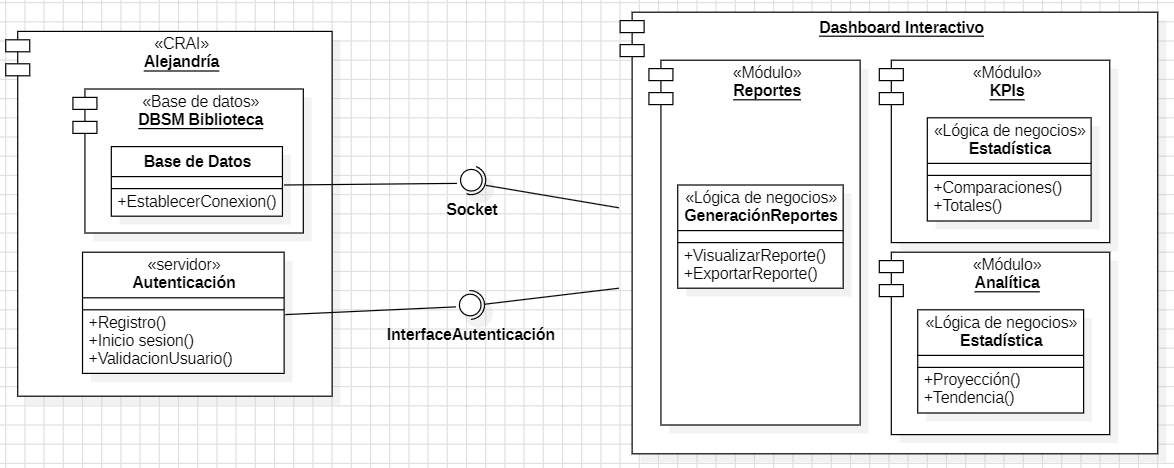
\includegraphics[width=0.9\linewidth]{img/Diagramas/dominio.png}
	\vspace{-1mm}
	\caption[Diagrama de dominio]{\textit{Diagrama de dominio del sistema.}}
	\label{fig:domain} 
\end{figure}

El usuario administrativo tiene acceso a los módulos respectivos una vez es autenticado. Para la conformación de los módulos, se consideró el diseño del \textit{backend} como su principal diferenciador. En la tabla \ref{tab:modulos_titulos} se presenta cómo están compuestos los módulos.

\vspace{0.3cm}
El módulo de \textbf{reportes}  se caracteriza por la generación de tablas dentro de la página web, estas presentan columnas que contienen información clave de cada caso. Su principal objetivo es desglosar de cada uno de los registros que correspondan al caso, poniendo a disposición la posibilidad de filtrar por cada una de las columnas generadas, y exportar dicho reporte como un archivo descargable .xlsX para ser ejecutado en la herramienta Excel. 

\vspace{0.3cm}
Por otro lado, el módulo de KPIs corresponde a la información en tiempo real que describe el estado de la biblioteca: comparaciones entre distintas métricas, cantidades totales y distribución del inventario. Su principal objetivo es dar una visión de alto nivel de la biblioteca.

\vspace{0.3cm}
El módulo de analítica corresponde a las estadísticas que presentan proyecciones y tendencias entre distintas métricas. Su análisis plantea la posibilidad de la toma de decisiones estratégicas basándose en datos reales. 

\begin{table}[H]
    \centering
    \caption[KPIs y reportes]{\bfseries KPIs y reportes seleccionados}
    \label{tab:modulos_titulos}
    \resizebox{\columnwidth}{!}{\begin{tabular}{lll} \hline
        \textbf{Módulo correspondiente} & \textbf{Título} \\ \hline
        KPIs  & Cantidad de libros en total en el inventario \\ 
        KPIs & Comparación de libros por facultad \\ 
        KPIs   & Distribución de géneros en el inventario\\ 
        KPIs   & Comparación de préstamos por facultad en un periodo de tiempo determinado \\ 
        KPIs   & Comparación de libros prestados por facultad en un periodo de tiempo determinado \\ 
        KPIs  & Comparación de libros por uso en sala en un periodo de tiempo determinado \\ 
        KPIs  & Comparación de préstamos por estudiante en un periodo de tiempo determinado \\ 
        KPIs   & Comparación de préstamos por rol \\ 
        Analítica  & Tendencia basada en las temáticas que más frecuentan los usuarios de la biblioteca  \\ 
        Analítica   & Tendencia basada en el criterio de búsqueda de la página de Alejandría.\\ 
        Analítica   & Proyección de préstamo de libros basado en los diez primeros libros más prestados.\\ 
        Reportes   & Libros sin utilizar\\ 
        Reportes   & Libros según estado\\ 
        Reportes   & Préstamos según tipo de usuario\\ \hline
    \end{tabular}}
    \vspace{2mm}
    \newline
    \small{KPIs y reportes seleccionados para los diferentes módulos.}
\end{table}

\subsubsection{Análisis de la base de datos de la biblioteca: }

Al momento de realizar el análisis de la base de datos de la biblioteca Benedicto XVI, el equipo de trabajo se dio cuenta que, actualmente, esta no cuenta con relaciones de llaves foráneas entre tablas. Tampoco existe documentación de la base de datos. Por este motivo, se realizó un diagrama de entidad-relación partiendo del script de creación de esta, y las relaciones establecidas en el diagrama se plantearon como relaciones lógicas, basándose en el análisis de cada una de las tablas y sus filas correspondientes. Si dentro de una tabla se encontraban filas identificadoras qu correspondían a otra tabla, se establecía una relación lógica.

\vspace{0.3cm}
Inicialmente, se realizó un diagrama incluyendo todas las tablas que se encontraban dentro de la base de datos. Posteriormente, se fueron eliminando las tablas que no se alineaban al alcance del proyecto, tablas de prueba o con información obsoleta, como es el caso de la hemeroteca. En la figura \ref{fig:entidad-relacion} se encuentra el diagrama resultante del análisis realizado por el equipo. 

\begin{figure}[H] 
	\centering
	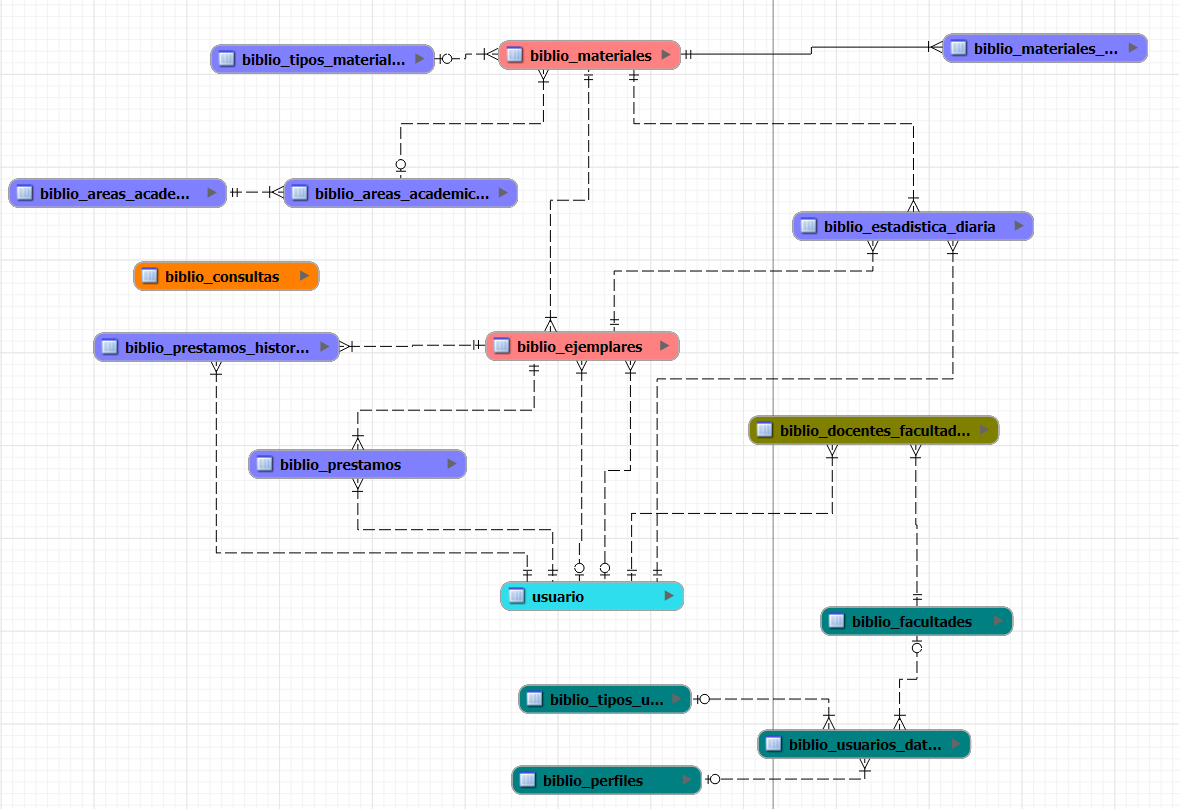
\includegraphics[width=0.8\linewidth]{img/Diagramas/entidad-relacion.png}
	\vspace{-1mm}
	\caption[Diagrama de entidad-relación de la base de datos de la biblioteca Benedicto XVI]{\textit{En el diagrama se contemplan únicamente las tablas utilizadas en el proyecto.}}
	\label{fig:entidad-relacion} 
\end{figure}
 
\vspace{0.3cm}
Como se había mencionado en secciones anteriores, la base de datos no posee una buena calidad en los datos almacenados. Entrando a fondo, se analiza el caso de las facultades registradas. 

\vspace{0.3cm}
Existen facultades repetidas dentro de la base de datos. En la figura \ref{fig:problemas-1}, se observa como la facultad de Ingeniería Eléctrica está registrada dos veces. Al hacer un análisis más profundo, se encuentra que ambas facultades tienen estudiantes asociados. La facultad de \textit{id} 43 presenta datos hasta la fecha del 2018, mientras que la facultad de \textit{id} 70 contempla datos hasta la actualidad. 

\vspace{0.3cm}
Esto genera un problema de inconsistencia que, si no es mitigado adecuadamente, podría propagarse en el resto del proyecto. La calidad de la información afecta seriamente la eficiencia y efectividad de un sistema \cite{DataQuality}.  

\vspace{0.3cm}
La información suele ser considerada de baja calidad si no es exacta, íntegra, consistente y actualizada\cite{DataQuality}. La información en la base de datos de la biblioteca falla en estos principios en gran porcentaje de sus registros.

 \begin{figure}[H] 
	\centering
	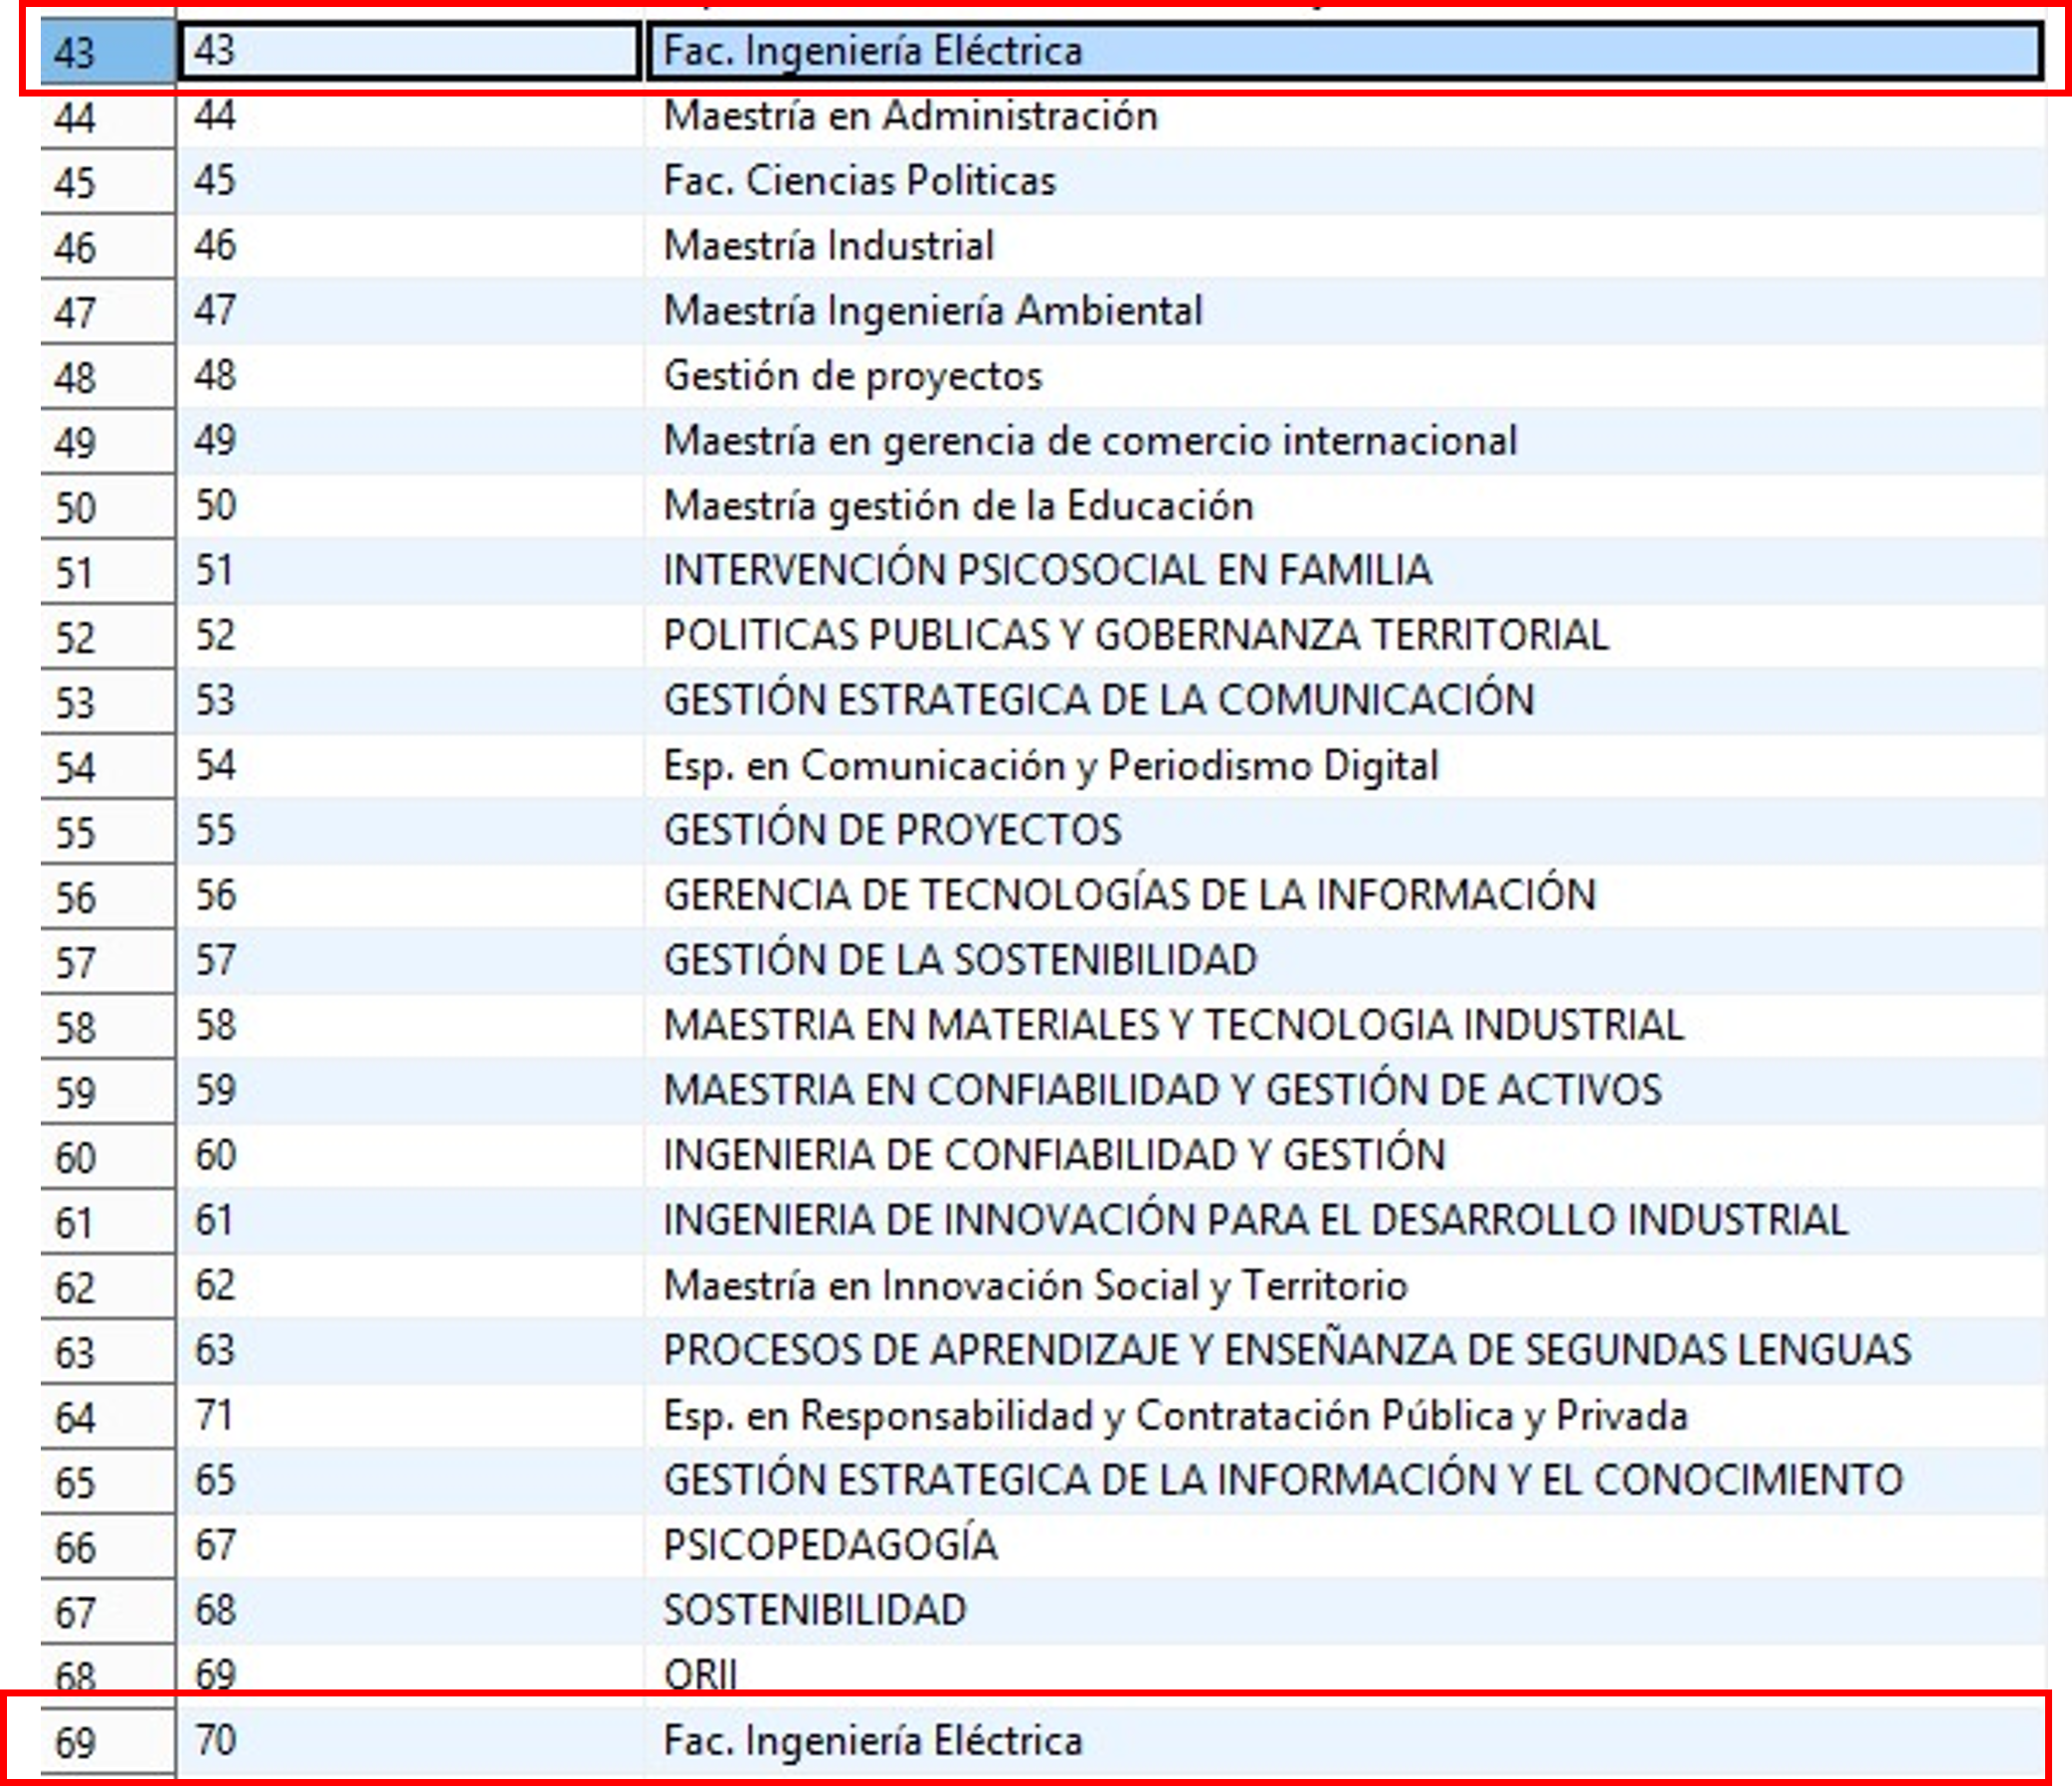
\includegraphics[width=0.8\linewidth]{img/variedades/bd-problemas1.png}
	\vspace{-1mm}
	\caption[Caso 1: Facultades en la base de datos repetidas]{\textit{La facultad de ingeniería Eléctrica está repetida en la base de datos.}}
	\label{fig:problemas-1} 
\end{figure}

El equipo de trabajo, tras consultarlo con el cliente, decidió trabajar con la facultad de \textit{id} 70, ya que está asociada a los registros actualizados. 

\vspace{0.3cm}
Como el caso de la facultad de ingeniería eléctrica, está el caso de la especialización de gestión de proyectos. Se encuentra duplicada en la base de datos, sin embargo, a diferencia de la facultad tratada en el caso anterior, esta no presenta estudiantes asociados en el registro duplicado. Se trabajó la facultad que tenía estudiantes asociados

\vspace{0.3cm}
Al analizar los registros de ejemplares y sus estados, el equipo de trabajo notó que en la base de datos existían errores tipográficos entre los distintos estados. En la figura \ref{fig:problemas-2} se encuentran los estados presentes.

 \begin{figure}[H] 
	\centering
	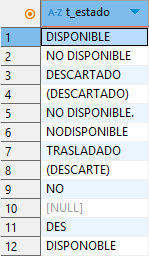
\includegraphics[width=0.2\linewidth]{img/variedades/bd-problemas2.png}
	\vspace{-1mm}
	\caption[Caso 2: Errores tipográficos en la base de datos]{\textit{En los estados de los ejemplares en la base de datos, se encuentran errores tipográficos}}
	\label{fig:problemas-2} 
\end{figure}

Se decidió junto con el cliente trabajar con los estados ''ACTIVO'', ''INACTIVO'', ''DESCARTADO'', ''TRASLADADO'', y el resto de estados agruparlos como ''EN REVISIÓN''. 


\subsection{Tercera fase: Diseño de las funcionalidades básicas del sistema }

\subsubsection{Cantidad de libros por estado y total: }

Esta medida contempla la cantidad de libros por estado en el inventario sin importar su estado en la base de datos. Se plantea el siguiente conjunto

\[
  \mathcal{E} \;=\; \{\, e_1,\,e_2,\,\dots,\,e_n \,\},
\qquad
\text{donde } n \text{ = número total de libros}
\]

Cada uno de los ejemplares presenta un atributo de estado, se define la pertenencia al grupo con todos los estados de la base de datos como:

\[
  \operatorname{estado}(e_i)\;\in\;
  \{\text{ACTIVO},\text{INACTIVO},\text{DESCARTADO},\text{TRASLADADO},\dots\}
\]

Y se define la función indicada, en donde si el ejemplar presenta el estado perteneciente al grupo se tomará el valor de 1, y 0 en el caso de no presentar estado seleccionado. 
\[
  \mathbf 1_{\{\operatorname{estado}(e_i)=s\}}
  \;=\;
  \begin{cases}
    1, & \text{si } \operatorname{estado}(e_i)=s,\\[4pt]
    0, & \text{en otro caso.}
  \end{cases}
\]
La sumatoria de libros con un estado S corresponde a:
\[
  N_s
  \;=\;
  \sum_{i=1}^{n}
    \mathbf 1_{\{\operatorname{estado}(e_i)=s\}}
  \quad
  \bigl(\text{total de libros con estado } s\bigr)
\]
En donde se sumará 1 cada vez que un ejemplar coincida con el estado S. Para calcular el total de libros sin importar el estado corresponde a:

\[
  N_{\text{total}}
  \;=\;
  \sum_{i=1}^{n} 1
  \;=\; n
  \quad
  \bigl(\text{total de libros sin importar estado}\bigr)
\]
Donde se sumará 1 sin importar el estado. 

%%%%%%%%5

\subsubsection{Comparación de libros por facultad:}
Esta medida compara la cantidad de libros totales por cada facultad, clasificándolos según su grupo de conocimiento de acuerdo al DDC. Para esta medida, la Jefatura de biblioteca otorgó una guía indicando a qué grupo de conocimiento correspondían las facultades de la universidad. En la tabla \ref{tab:ddc_facultades} se encuentra resumida esta información, y se anexó el ID correspondiente a las facultades planteadas. 

\addcontentsline{lot}{table}{\protect\numberline{\themytablecounter}Clasificación DDC según facultades de la universidad}
\begin{table}[H]
    
    \centering
    \caption[Clasificación DDC según facultades de la universidad]{\bfseries CLASIFICACIÓN DE DDC SEGÚN FACULTADES DE LA UNIVERSIDAD}
    \label{tab:ddc_facultades}
    \begin{tabular}{lll}
    
        \hline
        \textbf{ID Facultad} & \textbf{Nombre de la facultad} & \textbf{Inicial DDC} \\
        \hline
        7 & Ingeniería de Sistemas e Informática & 0 \\
        
        8, 24 & Psicología, Formación Humanística & 1 \\
        
        24 & Formación Humanística & 2 \\
        
        45, 10, 2 & Ciencias Políticas y Derecho & 3 \\
        
        23 & Idiomas & 4 \\
        
        22 & Ciencias Básicas & 5 \\
        
        3, 2, 4, 6, 1, 5, 27 \hspace{1cm} & Ingenierías y Negocios Internacionales\hspace{1cm} & 6 \\
        
        41 & Diseño Gráfico & 7 \\
        
        Aplica a todas & Aplica a todas & 8 \\
        
        Aplica a todas & Aplica a todas & 9 \\
        \hline
        
    \end{tabular}
    \vspace{2mm}
    
    \small{Estas son las diez principales clasificaciones del sistema Decimal Dewey alineado con las facultades de la universidad}
\end{table}

A partir de esto, se plantea la siguiente función 

\[
  d(e_i)\;=\;\text{primer dígito de la signatura Dewey de }e_i
  \quad (d\in\{0,\dots,9\}).
\]

donde \(e\) representa un libro, y \(d\) la pertenencia al conjunto del primer dígito de su decimal dewey. Se define el conjunto \(\alpha(d)\) para determinar la asociación de cada inicial del DDC con las facultades.

\[
  \alpha(d)=
  \begin{cases}
    \{7\}                         & d=0,\\
    \{8,24\}                      & d=1,\\
    \{24\}                        & d=2,\\
    \{45,10,2\}                   & d=3,\\
    \{23\}                        & d=4,\\
    \{22\}                        & d=5,\\
    \{3,2,4,6,1,5,27\}            & d=6,\\
    \{41\}                        & d=7,\\
    \text{todas las facultades}   & d=8,\\
    \text{todas las facultades}   & d=9.
  \end{cases}
\]

Para determinar la pertenencia al conjunto de la facultad \(F\) se plantea la siguiente función:
\[
  \mathbf 1_{\{F\in\alpha(d(e_i))\}} \;=\;
  \begin{cases}
    1, & \text{si la facultad }F\text{ pertenece a }\alpha\bigl(d(e_i)\bigr),\\
    0, & \text{en otro caso.}
  \end{cases}
\]
Por último, se plantea la sumatoria para cada una de las facultades, en donde se suma uno si la facultad \(F\) cumple con las condiciones de pertenencia al conjunto \(\alpha(d)\), según lo planteado en la función anterior. 
\[
  N_F
  \;=\;
  \sum_{i=1}^{n}
    \mathbf 1_{\{F\in\phi(d(e_i))\}}
  \quad
  \bigl(\text{total de ejemplares asignados a la facultad }F\bigr)
\]
%%%%%%%%%%%%%%%%%%%%%%%%%%55

\subsubsection{Comparación de grupos literarios: }
Compara las cantidades totales entre los diferentes grupos literarios de cada libro en el inventario actualizado de la biblioteca. Para esto se contempla el ejemplar \(e_i\) con su estado:

\[
  \operatorname{estado}(e_i)\; \; 
  \]

el primer dígito del DDC del ejemplar \(e_i\)
  \[
  d(e_i)\in\{0,\dots,9\},\; 
\]
  y este resultado se multiplica por 100, para obtener el grupo literario:
  \[
  r(e_i)=100\,d(e_i)\in\{0,100,\dots,900\}
  \]

Se plantean dos funciones para evaluar el ejemplar según su estado ''DISPONIBLE'' y la pertenencia al rango \(r\)

\[
  \mathbf 1_{\{\operatorname{estado}(e_i)=\text{DISPONIBLE}\}}
  \;=\;
  \begin{cases}
    1, & \text{si }e_i\text{ está DISPONIBLE},\\
    0, & \text{otro caso;}
  \end{cases}
\qquad
  \mathbf 1_{\{r(e_i)=r\}}
  \;=\;
  \begin{cases}
    1, & \text{si el rango de }e_i\text{ es }r,\\
    0, & \text{otro caso.}
  \end{cases}
\]

\[
  N_r
  \;=\;
  \sum_{i=1}^{n}
    \mathbf 1_{\{\operatorname{estado}(e_i)=\text{DISPONIBLE}\}}
    \cdot
    \mathbf 1_{\{r(e_i)=r\}}
  \quad
  \left(\text{total de ejemplares DISPONIBLES en el rango }r\right)
\]



%%%%%%%%%%%%%%%%%%%%%%%%%%%%%%555


\subsubsection{Comparación de préstamos por facultad:}
Se plantea como la comparación de la cantidad total de préstamos entre las diferentes facultades que hacen parte de la UPB. Se define \(P\) como la cantidad total de préstamos:

\[
  \mathcal{P}\;=\;\{
      p_1,p_2,\dots,p_m
  \}
\]

A partir de esto, se busca la facultad que corresponde a dicho préstamo. 

\[
  \operatorname{fac}(p_j)\;=\;\text{facultad del usuario que hizo el préstamo }p_i.
\]

Por lo tanto, se plantea una función en donde se evalúa si para la facultad del préstamo fac\((p_i)\) corresponde con la facultad \(F\) del caso. 

\[
  \mathbf 1_{\{\operatorname{fac}(p_i)=F\}}
  \;=\;
  \begin{cases}
    1, & \text{si } \operatorname{fac}(p_i)=F,\\[4pt]
    0, & \text{en otro caso.}
  \end{cases}
\]

A partir de esa función, se plantea la siguiente sumatoria para cada facultad:
\[
  N_F
  \;=\;
  \sum_{j=1}^{m}
    \mathbf 1_{\{\operatorname{fac}(p_j)=F\}}
  \quad
  \bigl(\text{total de préstamos registrados para la facultad }F\bigr).
\]


%%%%%%%%%%%%%%%%%%%%%%%%%%%%%%%
\subsubsection{Comparación de préstamos por tipo de usuario:}
Corresponde a comparar los préstamos entre los distintos usuarios de la base de datos. Estos préstamos tienen un usuario asociado, y cada usuario posee un rol. Se definen los roles de cada usuario en el siguiente conjunto:

\[
  \operatorname{rol}(p_i)\;\in\;
  \left\{
    \begin{aligned}
      &\text{Estudiante},\;\text{Docente},\;\text{Administrativo},\\
      &\text{Especializaciones},\;\text{Trabajo de grado},\;\text{Maestría},\\
      &\text{Práctica},\;\text{Externos},\;\text{Diplomados},\;\text{Egresado}
    \end{aligned}
  \right\}
\]

\vspace{0.3cm}

Se define \(P\) como la cantidad total de préstamos:

\[
  \mathcal{P}\;=\;\{
      p_1,p_2,\dots,p_m
  \}
\]

Por lo tanto, se plantea una función en donde se evalúa el tipo de usuario \(R\) de un préstamo \(p_i\):

\[
  \mathbf 1_{\{\operatorname{rol}(p_i)=R\}}
  \;=\;
  \begin{cases}
    1, & \text{si } \operatorname{rol}(p_i)=R,\\[4pt]
    0, & \text{en otro caso.}
  \end{cases}
\]

Se define la siguiente sumatoria para cada rol:
\[
  N_R
  \;=\;
  \sum_{j=1}^{m}
    \mathbf 1_{\{\operatorname{rol}(p_i)=R\}}
  \quad
  \bigl(\text{total de préstamos registrados para un rol }R\bigr).
\]

%%%%%%%%%%%%%%%%%%%%%%%%%%%%%%%%%%%%%%

\subsubsection{Comparación de libros prestados por facultad: }
Consiste en comparar el total de préstamos entre los diez libros más prestados de una facultad seleccionada.

Nuevamente, se define P como el conjunto de la cantidad total de préstamos:

\[
  \mathcal{P}\;=\;\{
      p_1,p_2,\dots,p_m
  \}
\]

Como se ha planteado anteriormente, cada préstamo tiene asociado un usuario, y este está asociado a una facultad de la universidad. 
\[
  \operatorname{fac}(p_i)          \;=\; \text{facultad del usuario de }p_i
\]

\[
  \operatorname{lib}(p_i)          \;=\; \text{libro prestado en }p_i
\]
Se evalúa la facultad \(F\) del usuario \(R\) de un préstamo \(p_i\). Posteriormente, de cada préstamo se extrae el libro prestado \(L\), y se suma 1 tanto al libro prestado asociado con la facultad correspondiente. 

\[
  N_{F,L}\;=\;
  \sum_{i=1}^{m}
    \mathbf 1_{\{\operatorname{fac}(p_i)=F\}}
    \;\mathbf 1_{\{\operatorname{lib}(p_i)=L\}}
\]

\[
  \text{(número total de veces que el libro }L\text{ fue prestado por usuarios de la facultad }F)
\]

Una vez se obtiene el total de la cantidad de préstamos de un libro \(L\) asociado según la facultad de los usuarios que lo prestaron, se filtran los primeros diez con más préstamos. 

\subsubsection{Comparación de libros por uso en sala: }
Consiste en comparar la cantidad de veces que han usado  los diez primeros libros que presenten más usos en la sala de la biblioteca. Se define el conjunto de los usos en sala como:


\[
  \mathcal{S}= \{\,s_1,s_2,\dots,s_k\,\}
  \quad\text{registro de los usos en sala}
\]

Cada libro usado en la sala por un usuario es registrado.
\[
  \operatorname{lib}(s_i)
  \;=\;
  \text{libro usado en el evento }s_i
\]

Se realiza un conteo de los libros que tienen registrados usos en la sala, y se suma 1 por cada libro.

\[
  N_{L}
  \;=\;
  \sum_{i=1}^{k}
    \mathbf 1_{\{\operatorname{lib}(s_i)=L\}}
  \quad
  \bigl(\text{veces que el libro }L\text{ fue usado en sala}\bigr)
\]

Una vez definida las cantidades en la que los libros fueron usados en sala, se filtra por los diez primeros libros más usados.

\subsubsection{Comparación de préstamos por estudiantes: }

Consiste en comparar la cantidad de libros prestados por los diez primeros usuarios con rol de estudiantes que registren más préstamos. 

Como en los anteriores casos, se define P como el conjunto de la cantidad total de préstamos:

\[
  \mathcal{P}\;=\;\{
      p_1,p_2,\dots,p_m
  \}
\]

Y como ya se había explicado, cada préstamo \(p\) tiene asociado un usuario el cual realizó dicho préstamo.
\[
  \operatorname{u}(p_i)
  = u_i
  \quad\text{usuario que realizó el préstamo }p_i
\]
 
Se evalúa el usuario del préstamo:
\[
  \mathbf 1_{\{\operatorname{u}(p_i)=u\}}
  = 
  \begin{cases}
    1, & \text{si el préstamo }p_i\text{ lo realizó el usuario }u,\\[4pt]
    0, & \text{en otro caso.}
  \end{cases}
\]

Se filtra por tipo de usuario \(u\), en este caso, el tipo de usuario sería estudiante.
\[
  \mathbf 1_{\{\operatorname{rol}(u)=\text{Estudiante}\}}
  =
  \begin{cases}
    1, & \text{si el usuario }u\text{ tiene rol “Estudiante”,}\\[4pt]
    0, & \text{en otro caso.}
  \end{cases}
\]

Para determinar la cantidad de préstamos por estudiante se establece la siguiente sumatoria: 
\[
  N_{u}
  =
  \sum_{i=1}^{m}
     \mathbf 1_{\{\operatorname{usr}(p_i)=u\}}
     \cdot
     \mathbf 1_{\{\operatorname{rol}(u)=\text{Estudiante}\}}
  \quad
  \bigl(\text{número de préstamos hechos por el estudiante }u\bigr)
\]

\vspace{0.3cm}
Por otro lado, se plantean las siguientes propuestas para el \textbf{módulo de reportes:}

\subsubsection{Libros que no han sido usado en años: }Para esto, se plantea una consulta en donde verifique los libros que no han sido usados en un periodo de más de cinco años.
\subsubsection{Libros según su estado: } Corresponde a los libros que poseen un estado distinto de "DISPONIBLE", de manera que se ofrece el detalle de estos y sus estados registrados.
\subsubsection{Préstamos por tipo de usuario:} Muestra los préstamos por cada tipo de usuario indicando la facultad o departamento al que pertenezca.

\vspace{0.3cm}
Por último, para el \textbf{módulo de analítica}, se plantean la Tendencia basada en el criterio de búsqueda de la página de Alejandría, la proyección de préstamo de libros basado en los diez primeros libros más prestados y Tendencia basada en las temáticas que más frecuentan los usuarios de biblioteca. Esta información se trabajará con una muestra de los veinticuatro meses anteriores a partir del mes de consulta. La proyección se realizará a seis meses.

\vspace{0.3cm}
%%%%%%%%%%%%%%TERCERA ENTREGA
\subsection{Cuarta fase: Diseño del prototipo}

A partir del análisis del problema y el diseño de las funcionalidades preliminar, se realiza el diseño del prototipo. Esta fase es supervisada por jefatura de biblioteca.

\subsubsection{Planteamiento de historias de usuario: }

Las historias de usuario definidas se encuentran dentro del APÉNDICE \ref{APÉNDICE:a}. Fueron supervisadas por el director del proyecto de grado y aprobadas por jefatura de biblioteca, alineándose con el primer objetivo planteado para el proyecto.

\subsubsection{Planteamiento de requerimientos del sistema: }

Una vez establecidas las historias de usuario, se realizó el documento de requerimientos de software, el cual se encuentra adjunto en el APÉNDICE \ref{APÉNDICE:a}. El documento fue revisado por el director ded proyecto de grado, y aprobado por jefatura de biblioteca, cumpliendo el primer objetivo planteado para el proyecto. 

\subsubsection{Diseño inicial UX del sistema: }
Se presentó al cliente un diseño inicial del sistema. Este diseño fue aprobado, sin embargo, durante la fase de desarrollo sufrió distintos cambios, a medida que iba siendo supervisado por el director del trabajo de grado y el cliente. En en apéndice \ref{APÉNDICE:B} se encuentra el diseño de este. Este se alinea con lo planteado en el segundo objetivo del proyecto. 

%%%%%%%%%%%%%%%%%%%%%%%%%%%%%%%%%%%5
\subsection{Quinta fase: Desarrollo del prototipo e implementación}

La fase de desarrollo está enmarcada por el marco de trabajo Scrum. Se realizaron tres Sprints de trabajo. 
En el apéndice \ref{APÉNDICE:C} se encuentra la documentación correspondiente a la estructura y comportamiento del sistema desarrollado.

 
 \subsubsection[Primer Sprint]{Primer Sprint: }
 El objetivo del primer Sprint corresponde a la fase de desarrollo del módulo de KPIs, tanto sus funcionalidades como el apartado gráfico. Las historias comprometidas
 para este sprint corresponden a las relacionadas al módulo de KPIs, y la historia designada para escoger un rango de fechas definido por el usuario.
 A continuación, se presenta una gráfica con los puntos comprometidos y la deuda técnica. 

\begin{figure}[htpb] 
	\centering
	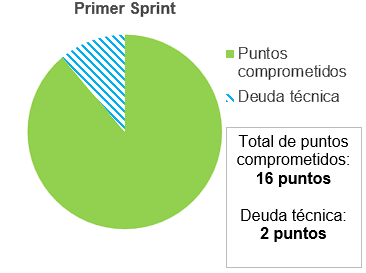
\includegraphics[width=0.4\linewidth]{img/Sprints/S1.png}
	\vspace{-1mm}
	\caption[Puntos comprometidos primer Sprint]{\textit{Puntos comprometidos para el Primer Sprint. Imagen propia}}
	\label{fig:S1} 
\end{figure}

La deuda técnica corresponde a la historia relacionada con escoger un rango de fechas definido por el usuario. Esta historia se comprometió para el siguiente Sprint. 
La velocidad del equipo en este sprint fue de 80\%.

\begin{figure}[htpb] 
	\centering
	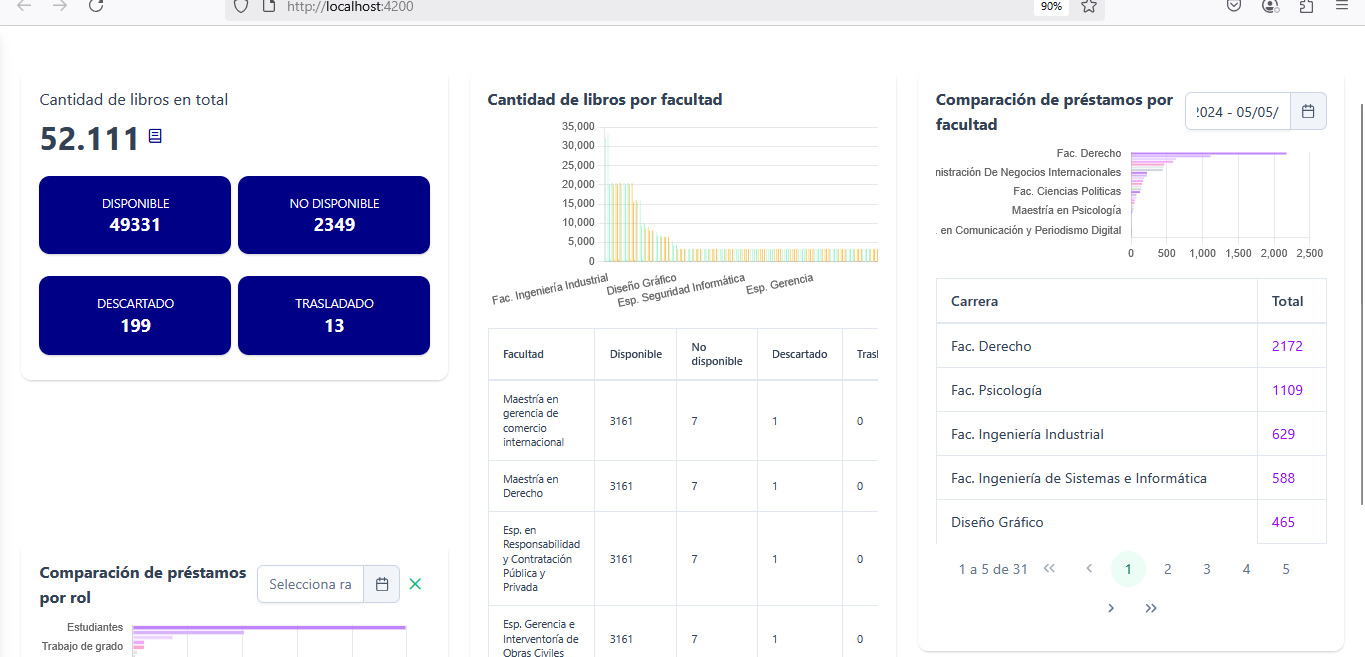
\includegraphics[width=0.8\linewidth]{img/UX/s1-1.jpg}
	\vspace{-1mm}
	\caption[Primera versión software]{\textit{Primera versión software. Imagen propia}}
	\label{fig:S1-1} 
\end{figure}

La figura \ref{fig:S1-1} corresponde a una muestra de la primera iteración del software. En el sprint review, se obtuvo retroalimentación
por parte del cliente. Estas recomendaciones se plantearon para el siguiente sprint. 


\subsubsection[Segundo Sprint]{Segundo Sprint: }

 Para el segundo sprint se planteó como objetivo el desarrollo del módulo de reportes, y se asumió la deuda técnica del sprint anterior. Por lo tanto, 
 la historias comprometidas corresponden al módulo de reportes. La siguiente gráfica presenta los puntos comprometidos para el sprint.


\begin{figure}[htpb] 
	\centering
	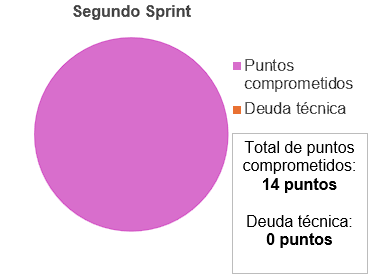
\includegraphics[width=0.4\linewidth]{img/Sprints/S2.png}
	\vspace{-1mm}
	\caption[Puntos comprometidos segundo Sprint]{\textit{Puntos comprometidos para el Segundo Sprint. Imagen propia}}
	\label{fig:S2} 
\end{figure}

Se cumplió con la totalidad de puntos, dando como resultado una velocidad de equipo del 100\%. Aparte, se adaptó el prototipo
según la retroalimentación del cliente, dando como resultado la segunda iteración de este.

\begin{figure}[htpb] 
	\centering
	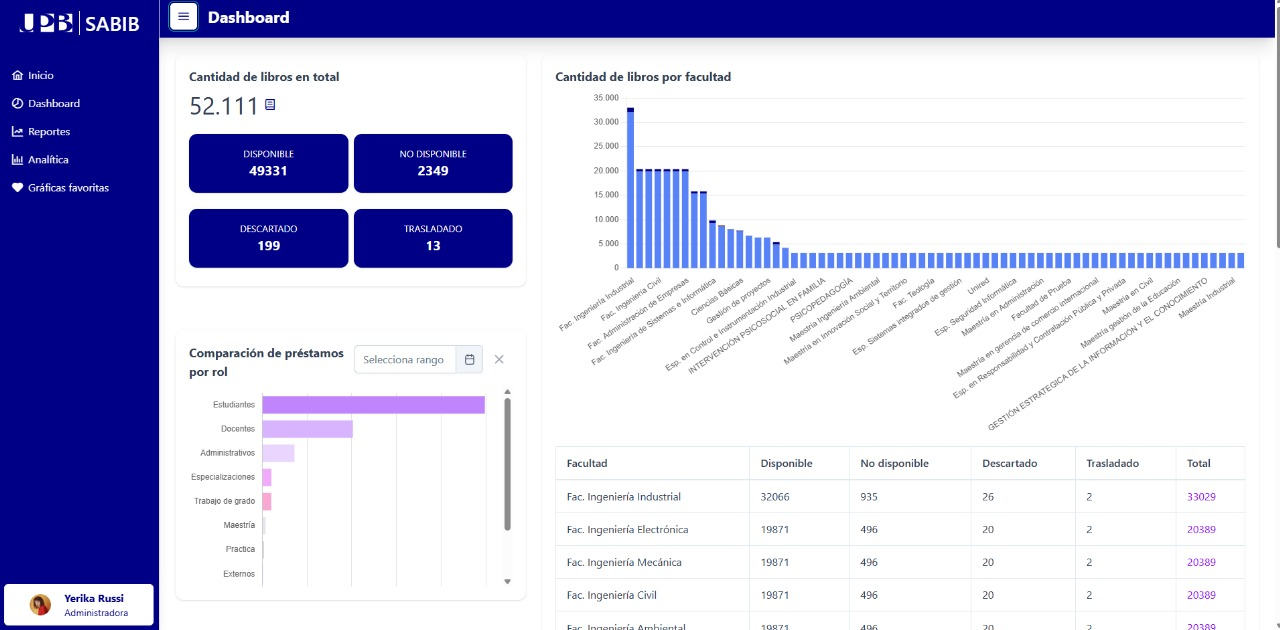
\includegraphics[width=0.8\linewidth]{img/UX/s2-1.jpg}
	\vspace{-1mm}
	\caption[Segunda iteración del software]{\textit{Segunda iteración del software. Imagen propia}}
	\label{fig:S2-1} 
\end{figure}

En el sprint review, el cliente realizó la debida retroalimentación, haciendo énfasis en la necesidad de usar la gama
de colores institucionales. Estas observaciones se consideraron de alta prioridad.

\subsubsection[Tercer Sprint]{Tercer Sprint: }

En el tercer sprint se comprometieron las historias relacionadas al módulo de analítica, realizar la función de añadir 
gráficas a favoritos y aplicar la paleta de colores institucionales al software. Se obtuvo la siguiente gráfica de puntos comprometidos:

\begin{figure}[htpb] 
	\centering
	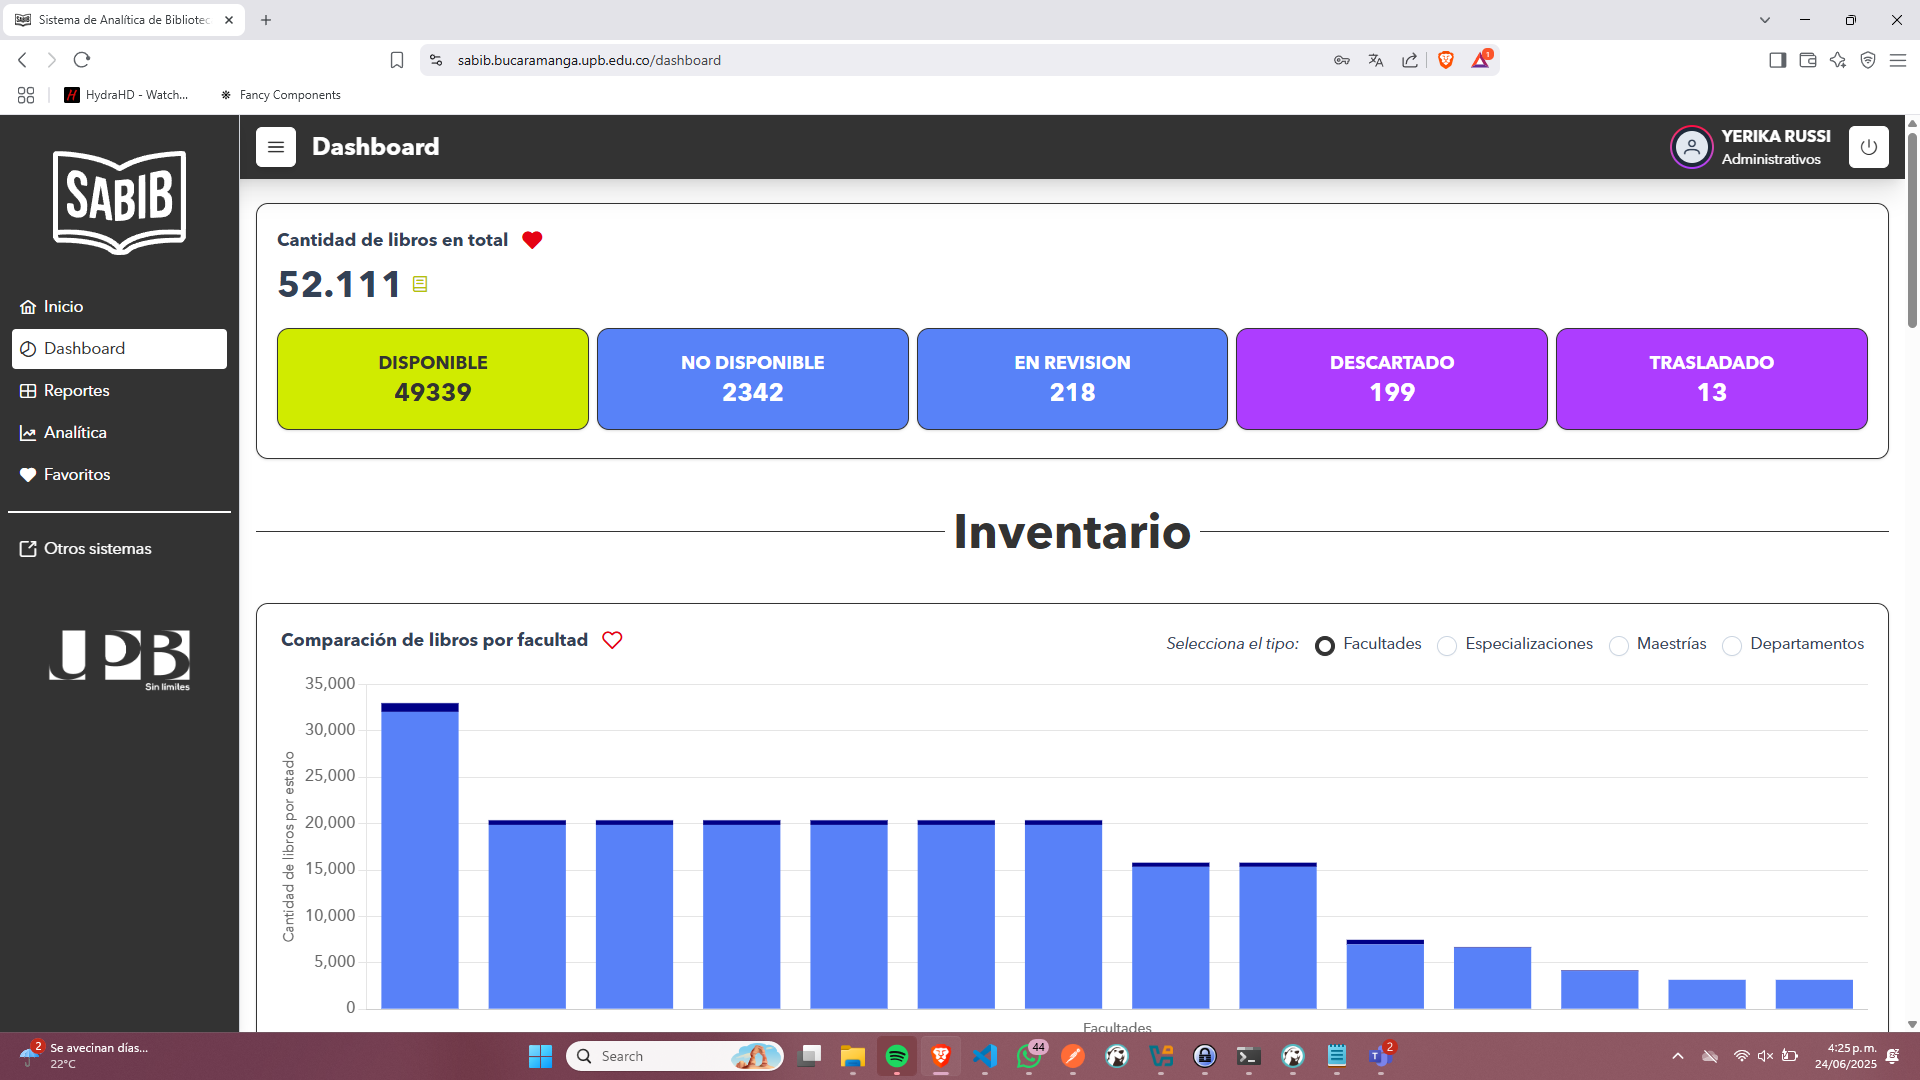
\includegraphics[width=0.8\linewidth]{img/UX/s3-1.png}
	\vspace{-1mm}
	\caption[Tercera iteración del software]{\textit{Tercera iteración del software. Imagen propia}}
	\label{fig:S3-1} 
\end{figure}

\subsubsection[Implementación]{Implementación y despliegue: }

Una vez el prototipo final fue aprobado por el cliente, el aplicativo se desplegó en una máquina virtual de sistema operativo Red Hat 9 dentro de la infraestructura de la universidad Pontificia Bolivariana.
Para el despliegue se empleó un archivo tipo \textit{bash}. El departamento de CTIC de la institución ejecutó el archivo correspondiente después de una revisión
de seguridad de este. El departamento de CTIC limitó el acceso al aplicativo, permitiendo solo tráfico que provenga de las redes LAN institucionales. 

\vspace{0.3cm}
En el apéndice \ref{APÉNDICE:D} se encuentra adjunto pruebas del aplicativo desplegado en el dominio \textit{sabib.bucaramanga.upb.edu.co}, demostración de sus funcionalidades y una prueba de conectividad realizada a los puertos 3000 (el cual corresponde al 
servidor del \textit{backend}) y 443 (el cual corresponde al servidor del \textit{frontend}). Por otro lado,
en el apéndice \ref{APÉNDICE:E} se encuentra la carta de entrega, firmada por los 
integrantes del equipo y jefatura de biblioteca.



% Conclusiones
\newpage
\section{CONCLUSIONES}
\begin{itemize}
  \item Las reuniones semanales con el cliente fueron claves para mantener el foco durante la planeación y desarrollo del proyecto, permitiendo la priorización de tareas según las necesidades del usuario final.
  \item El diseño de artefactos como los middlewares, y la utilización de interfaces como express router sirvieron para la reutilización de código, agilizando el desarrollo del proyecto y permitiendo cumplir con el cronograma planteado.
  \item El uso del marco de trabajo Scrum al momento del desarrollo permitió la adaptación del prototipo por medio de ciclos iterativos, incorporando las observaciones realizadas por el cliente en cada revisión y agregando las funcionalidades correspondientes a cada módulo comprometido. 
  \item La adaptación de una metodología para el desarrollo de dashboards  permitió la organización del proyecto en cinco fases, definiendo cada una de estas con actividades puntuales y metas medibles, dando como resultado un proyecto estructurado y entregables que se alinean a estas etapas y los objetivos planteados.


\end{itemize}
% Recomendaciones
\newpage
\section{RECOMENDACIONES}
Dentro de las recomendaciones que se realizan a partir del proyecto, se encuentran las siguientes:
\begin{itemize}
  \item Leer la documentación del proyecto en caso de retomarlo con el propósito de expandirlo, para que las decisiones que se tomen sean informadas, se mantenga coherencia con la arquitectura implementada y se eviten inconvenientes que puedan surgir por falta de familiarización con el sistema.
  \item Si se decide realizar cambios en el sistema, al momento de desplegar este proyecto en la infraestructura de la universidad, se recomienda diseñar un archivo bash, el cual permita automatizar el proceso de instalación de dependencias y la configuración del entorno. Se deja un ejemplo de archivo en los entregables del proyecto, con el fin de que sirva como guía para futuras implementaciones.
  \item Centralizar la autenticación para los distintos sistemas propios de la universidad, debido a que, en tal caso de que se realicen acciones no previstas, se tendrían que realizar múltiples actualizaciones a los sistemas que se encuentren en producción, lo que podría generar inconsistencia, aumentar el riesgo de errores y generar problemas de escalabilidad.
  \item Integrar el sistema de biblioteca Alejandría, junto con el sistema SABIB, con el fin de que el usuario pueda acceder a los servicios de ambos sistemas con una sola autenticación, buscando la centralización.
  \item Debido a que dentro de la base de datos actual no se encuentran normalizados los estados de los libros en el inventario, se recomienda que se realice la implementación de una tabla que los especifique, con el fin de evitar inconsistencias a la hora de realizar consultas, mejorando la calidad de los datos almacenados.
  \item Remover las tablas que no se encuentren en uso dentro de la base de datos, para mejorar la mantenibilidad y legibilidad de los datos almacenados.
  \item En caso de realizar una migración de la base de datos, se recomienda actualizar los queries del backend, ya que estos están adaptados para MySQL 5 y podrían presentar problemas de compatibilidad y rendimiento con versiones más recientes.
\end{itemize}

\newpage
\renewcommand\refname{REFERENCIAS}

\newpage
\renewcommand\refname{REFERENCIAS}
\bibliographystyle{IEEEtran}
\bibliography{bibliography.bib}
\addcontentsline{toc}{section}{REFERENCIAS}

% APÉNDICES
\newpage
\addcontentsline{toc}{section}{APÉNDICES}
\begin{center}
\textbf{APÉNDICES}
\end{center}
\appendix

%%%%%%%%%%%%%APENDICE A
\raggedright\textit{\textbf{APÉNDICE A} RESULTADOS DEL PRIMER OBJETIVO}
\label{APÉNDICE:a}

A continuación, en las siguientes páginas, se encuentran los documentos que corresponden a las historias de usuario planteadas para el sistema, y la especificación de requerimientos de este. 


\includepdf[pages=-, fitpaper]{img/PDF/UX_STORIES_FINAL_OBJ1.pdf}
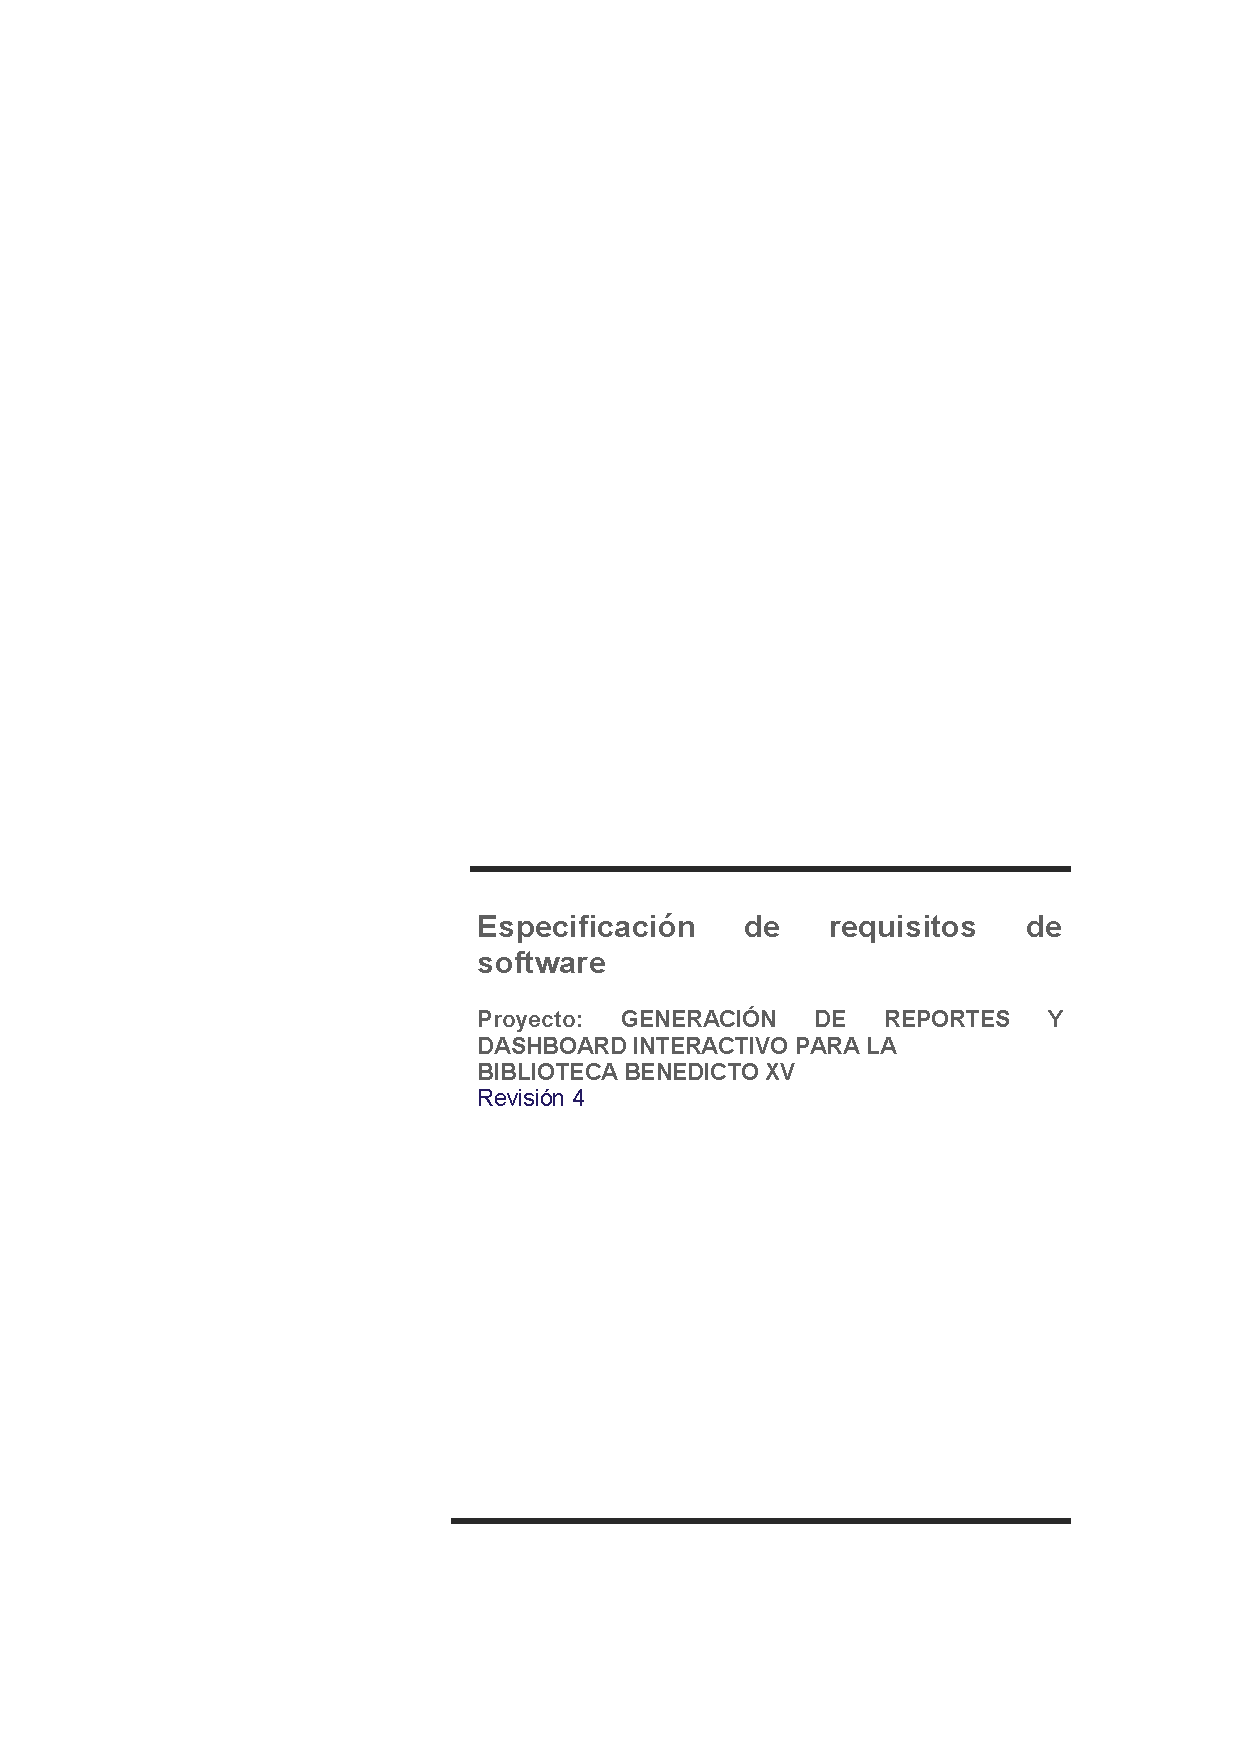
\includepdf[pages=-, fitpaper]{img/PDF/ESP_REQ_FINAL_OBJ1.pdf}


%%%%%%%%%%%%%APENDICE B
\raggedright\textit{\textbf{APÉNDICE B} RESULTADOS DEL SEGUNDO OBJETIVO}
\label{APÉNDICE:B}

A continuación, en las siguientes páginas, se encuentra el diseño de la interfaz de usuario, basándose en los requerimientos propuestos. 

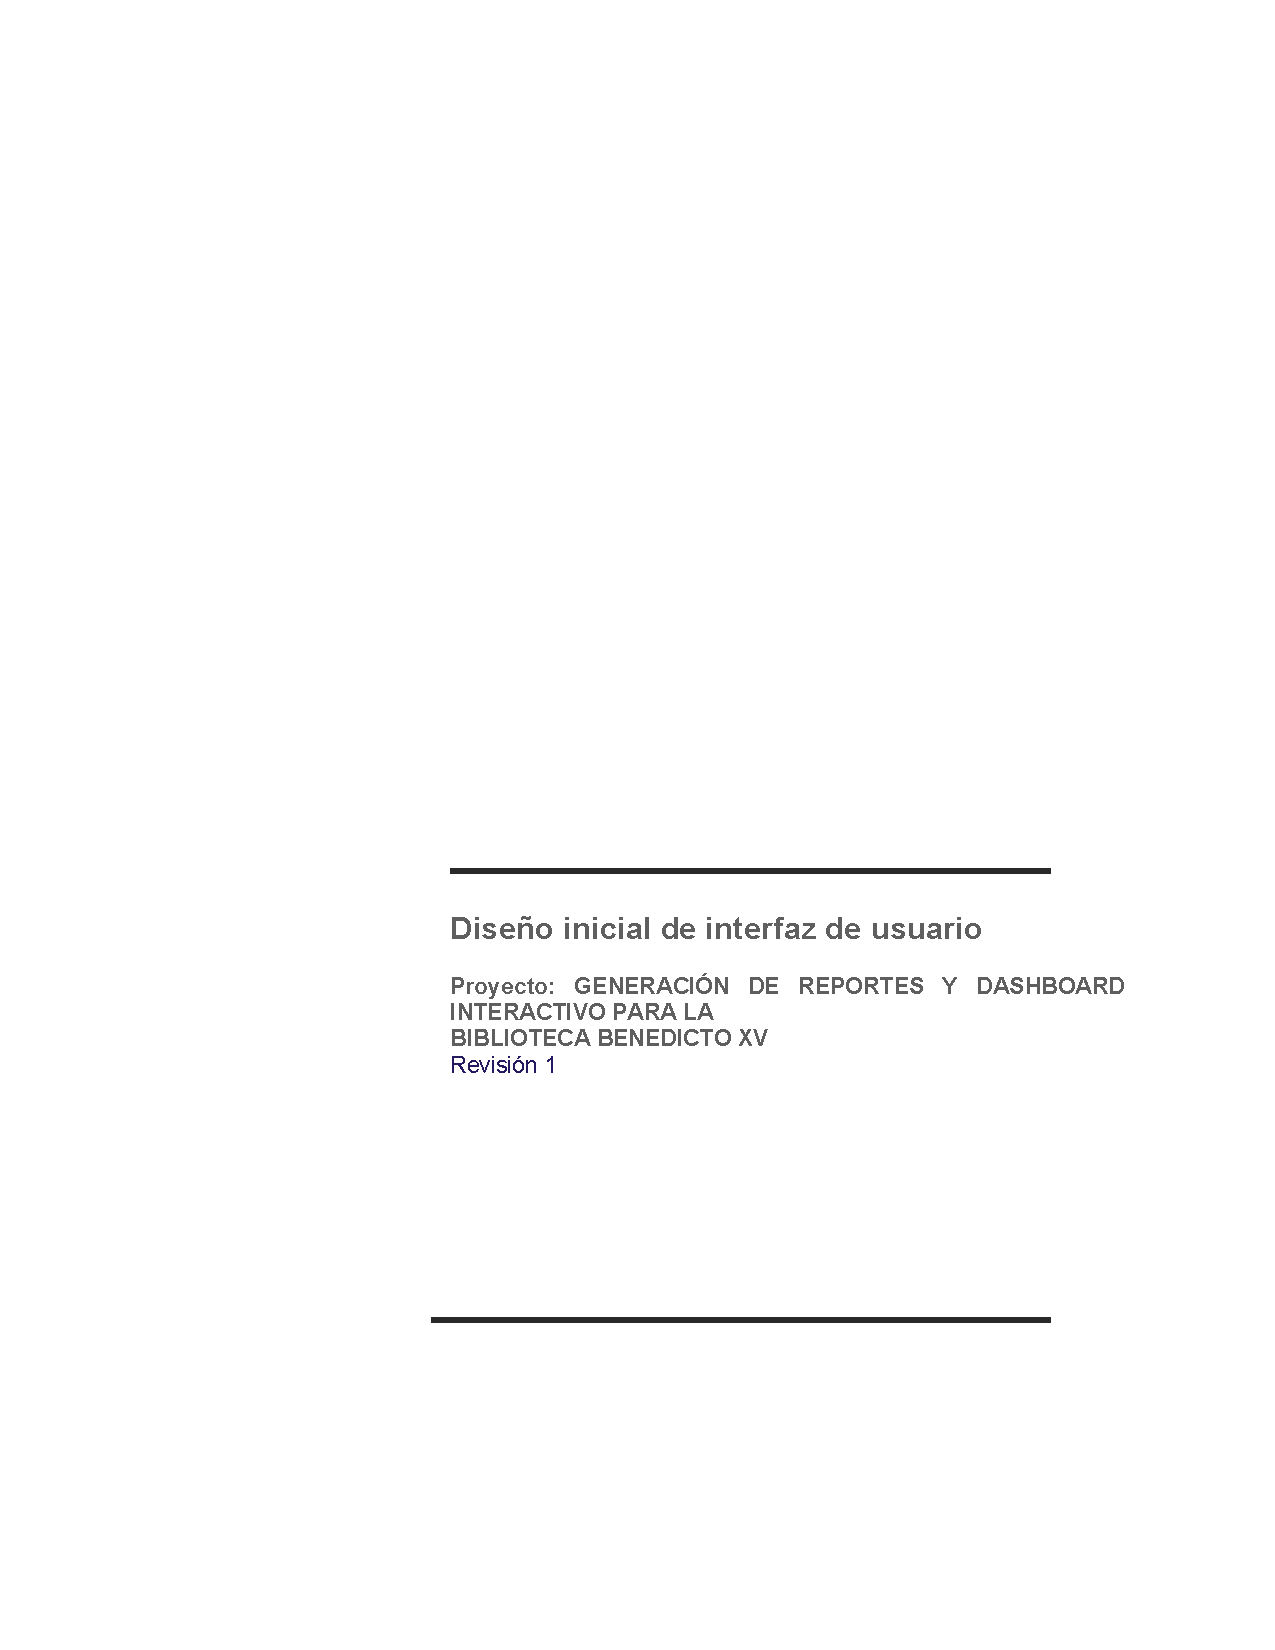
\includepdf[pages=-, fitpaper]{img/PDF/UX_DESIGN_OBJ2.pdf}

%%%%%%%%%%%%%%%%%%%%%%%%%APENDICE C
\raggedright\textit{\textbf{APÉNDICE C} RESULTADOS DEL TERCER OBJETIVO}
\label{APÉNDICE:C}

En las siguientes páginas se encuentra la documentación referente a la estructura y comportamiento
del aplicativo.  

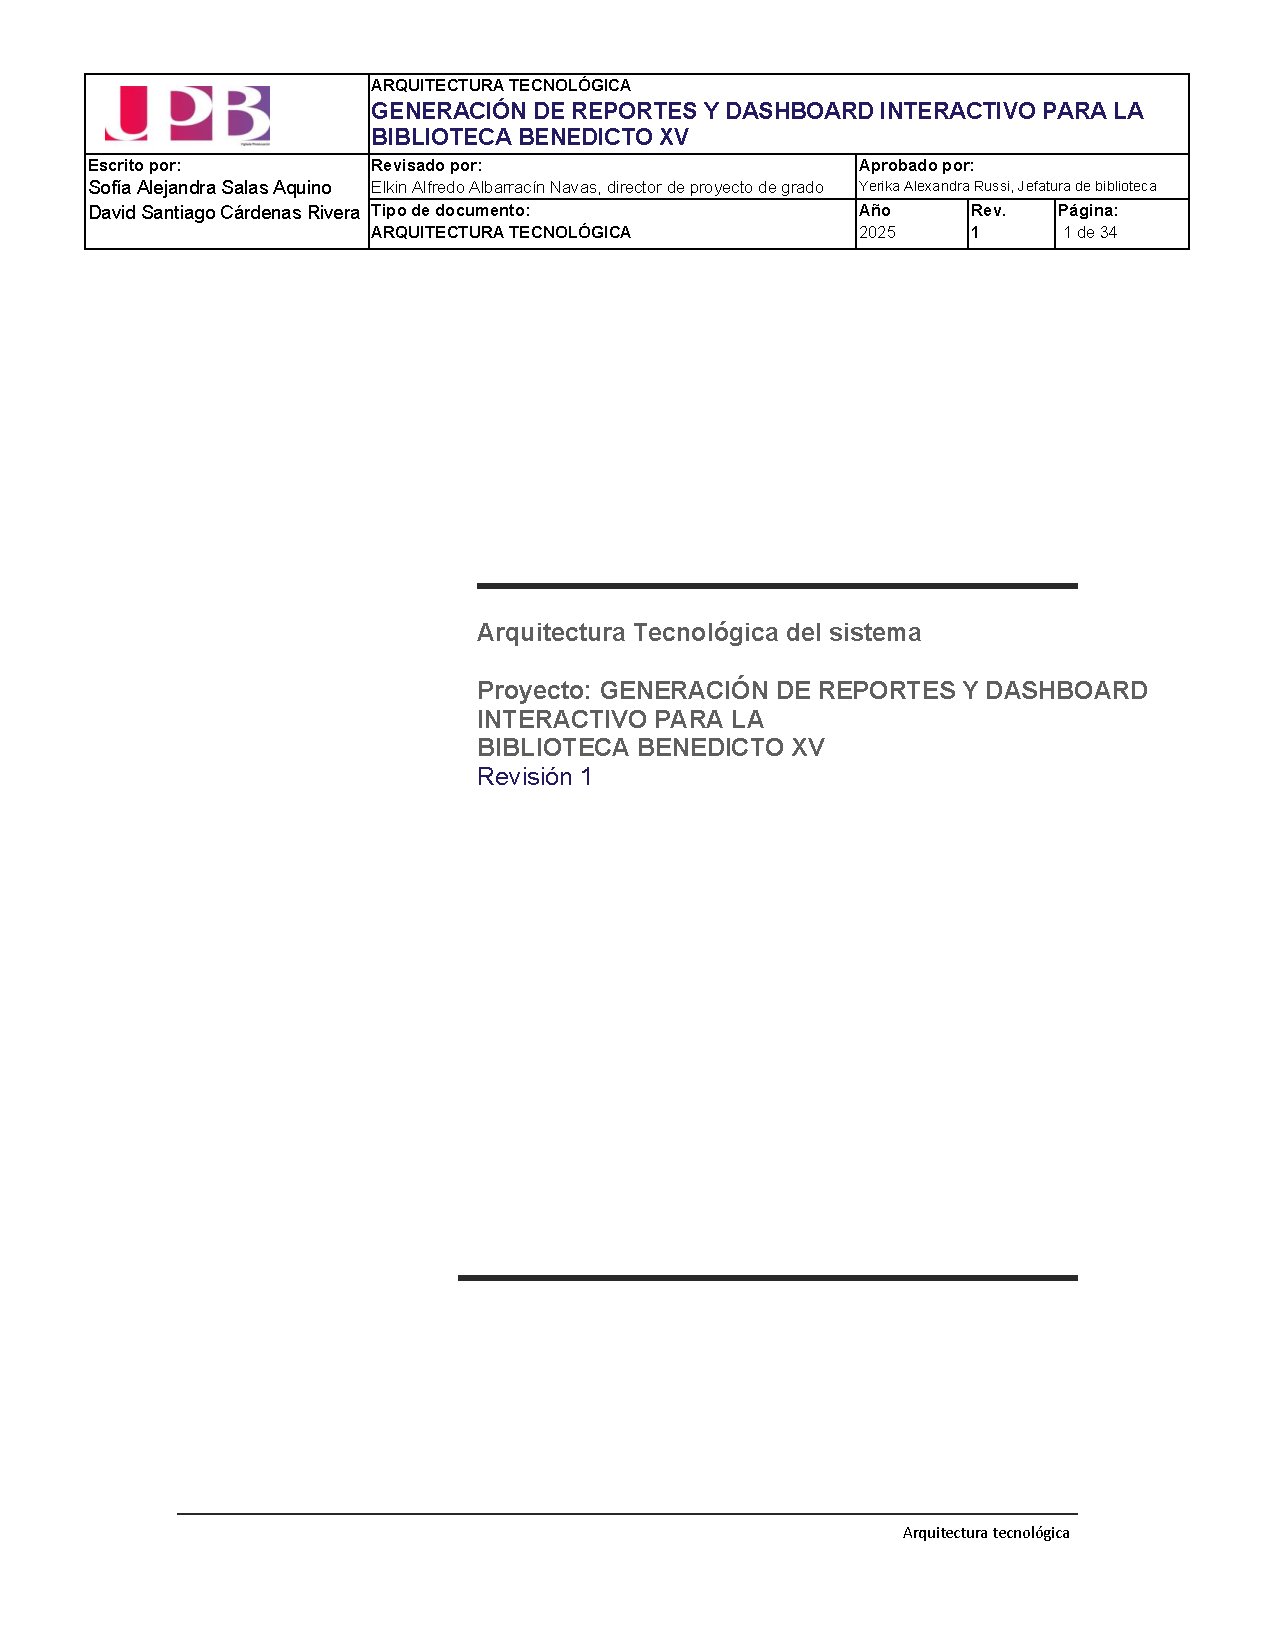
\includepdf[pages=-, fitpaper]{img/PDF/ESP_ARQ.pdf}

%%%%%%%%%%%%%APENDICE D
\raggedright\textit{\textbf{APÉNDICE D} RESULTADOS DEL CUARTO OBJETIVO}
\label{APÉNDICE:D}

A continuación, en las siguientes páginas, se encuentra el aplicativo final y una prueba de conectividad a los servidores donde se encuentra alojado, siguiendo lo planteado en la fase de planeación del proyecto, y las recomendaciones realizadas por los \textit{Stakeholders}. 

\includepdf[pages=-, fitpaper]{img/PDF/RESULTADOS-SOFTWARE.pdf}


%%%%%%%%%%%%%%%%%%CARTA
\raggedright\textit{\textbf{APÉNDICE E} CARTA DE ENTREGA}
\label{APÉNDICE:E}

A continuación, se encuentra la carta de entrega del proyecto. 

\includepdf[pages=-, fitpaper]{img/PDF/Carta-entrega.pdf}
\end{document}
